% MODELO LATEX PARA TCC DO IFCE 
% ELABORADO POR CARINA TEIXEIRA DE OLIVEIRA
% SETEMBRO DE 2017

\documentclass[
12pt, % tamanho da fonte
openright, % capítulos começam em pág ímpar (insere página vazia caso preciso)
oneside, % para impressão somente frente. Oposto a twoside (frente e verso)
a4paper, % tamanho do papel. 
% 	% -- opções do pacote babel --
english,% idioma adicional para hifenização
%french,% idioma adicional para hifenização
%spanish,% idioma adicional para hifenização
brazil,	% o último idioma é o principal do documento
]{abntex2}

% ------------------------
% PACOTES
% Mapear caracteres especiais no PDF
\usepackage{cmap}
% Usa a fonte Latin Modern
\usepackage{times}			
% Selecao de codigos de fonte.
\usepackage[T1]{fontenc}		
% Codificacao do documento (conversão automática dos acentos)
\usepackage[utf8]{inputenc}		
% Indenta o primeiro parágrafo de cada seção.
\usepackage{indentfirst}		
% Controle das cores
\usepackage{color}
\usepackage{soulutf8}
% Inclusão de gráficos
\usepackage{graphicx}			
\usepackage{multicol}
\usepackage{multirow}
% Criação de tabelas
\usepackage{longtable}
\usepackage{booktabs}
\newcommand{\tabitem}{~~\llap{\textbullet}~~} % item falso de lista
% \usepackage{booktabs}
%capitulos
\usepackage{titlesec}
% Pacotes adicionais, usados apenas no âmbito do Modelo Canônico do abnteX2
% para geração de dummy text
\usepackage{lipsum}				
% Pacotes de citações
% Paginas com as citações na bibl
\usepackage[brazilian,hyperpageref]{backref}	 
% Citações padrão ABNT
\usepackage[alf]{abntex2cite}	
% Pacote para definir cor nas tabelas
\usepackage[table,xcdraw]{xcolor}
% Pacote usado para exibir blocos de códigos de programação
\usepackage{listings}
\usepackage{chngcntr}
\lstset{frame=Trbl,numbers=left}
\renewcommand{\lstlistingname}{Exemplo}
\renewcommand{\lstlistlistingname}{Lista de \lstlistingname s}
% Pacote e configurações para quadros
\newcommand{\quadroname}{Quadro}
\newcommand{\listofquadrosname}{Lista de Quadros}
\newfloat{quadro}{loq}{\quadroname}
\setfloatadjustment{quadro}{\centering}
\newlistof{listofquadros}{loq}{\listofquadrosname}
\newlistentry{quadro}{loq}{0}
\renewcommand{\cftquadroname}{\quadroname\space}
\renewcommand{\cftquadroaftersnum}{\hfill\textendash\hfill}
% Pacote para incluir pdf
\usepackage{pdfpages}
% Definindo as linguagens a serem exibidas com lstlisting
\definecolor{mediumgray}{rgb}{0.3, 0.4, 0.4}
\definecolor{mediumblue}{rgb}{0.0, 0.0, 0.8}
\definecolor{forestgreen}{rgb}{0.13, 0.55, 0.13}
\definecolor{darkviolet}{rgb}{0.58, 0.0, 0.83}
\definecolor{royalblue}{rgb}{0.25, 0.41, 0.88}
\definecolor{crimson}{rgb}{0.86, 0.8, 0.24}
\colorlet{punct}{red!60!black}
\definecolor{background}{HTML}{EEEEEE}
\definecolor{delim}{RGB}{20,105,176}
\colorlet{numb}{magenta!60!black}
\definecolor{json_base}{RGB}{0,50,0}
\definecolor{codegreen}{rgb}{0,0.6,0}
\definecolor{codegray}{rgb}{0.5,0.5,0.5}
\definecolor{codepurple}{HTML}{C42043}
\definecolor{backcolour}{HTML}{F2F2F2}
\definecolor{bookColor}{cmyk}{0,0,0,0.90}  
\color{bookColor}

\lstdefinelanguage{JavaScript}{
  morekeywords=[1]{break, continue, delete, else, for, function, if, in,
    new, return, this, typeof, var, void, while, with},
  % Literals, primitive types, and reference types.
  morekeywords=[2]{false, null, true, boolean, number, undefined,
    Array, Boolean, Date, Math, Number, String, Object},
  % Built-ins.
  morekeywords=[3]{eval, parseInt, parseFloat, escape, unescape},
  sensitive,
  morecomment=[s]{/*}{*/},
  morecomment=[l]//,
  morecomment=[s]{/**}{*/}, % JavaDoc style comments
  morestring=[b]',
  morestring=[b]"
}[keywords, comments, strings]

\lstdefinelanguage[ECMAScript2015]{JavaScript}[]{JavaScript}{
  morekeywords=[1]{await, async, case, catch, class, const, default, do,
    enum, export, extends, finally, from, implements, import, instanceof,
    let, static, super, switch, throw, try},
  morestring=[b]` % Interpolation strings.
}

\lstalias[]{ES6}[ECMAScript2015]{JavaScript}

\lstdefinestyle{JSES6Base}{
  backgroundcolor=\color{white},
  basicstyle=\ttfamily,
  breakatwhitespace=false,
  breaklines=false,
  %captionpos=b,
  columns=fullflexible,
  commentstyle=\color{mediumgray}\upshape,
  emph={},
  emphstyle=\color{crimson},
  extendedchars=true,  % requires inputenc
  fontadjust=true,
  frame=single,
  identifierstyle=\color{black},
  keepspaces=true,
  keywordstyle=\color{mediumblue},
  keywordstyle={[2]\color{darkviolet}},
  keywordstyle={[3]\color{royalblue}},
  numbers=left,
  numbersep=5pt,
  numberstyle=\tiny\color{black},
  rulecolor=\color{black},
  showlines=true,
  showspaces=false,
  showstringspaces=false,
  showtabs=false,
  stringstyle=\color{forestgreen},
  tabsize=2,
  title=\lstname,
  upquote=true  % requires textcomp
}

\lstdefinestyle{JavaScript}{
  language=JavaScript,
  style=JSES6Base
}
\lstdefinestyle{ES6}{
  language=ES6,
  style=JSES6Base
}

\lstdefinelanguage{json}{
    basicstyle=\color{json_base}\normalfont\ttfamily,
    numbers=left,
    numberstyle=\scriptsize,
    stepnumber=1,
    numbersep=8pt,
    showstringspaces=false,
    breaklines=true,
    frame=single,
    backgroundcolor=\color{white},
    %captionpos=b,
    literate=
     *{0}{{{\color{numb}0}}}{1}
      {1}{{{\color{numb}1}}}{1}
      {2}{{{\color{numb}2}}}{1}
      {3}{{{\color{numb}3}}}{1}
      {4}{{{\color{numb}4}}}{1}
      {5}{{{\color{numb}5}}}{1}
      {6}{{{\color{numb}6}}}{1}
      {7}{{{\color{numb}7}}}{1}
      {8}{{{\color{numb}8}}}{1}
      {9}{{{\color{numb}9}}}{1}
      {:}{{{\color{punct}{:}}}}{1}
      {,}{{{\color{punct}{,}}}}{1}
      {\{}{{{\color{delim}{\{}}}}{1}
      {\}}{{{\color{delim}{\}}}}}{1}
      {[}{{{\color{delim}{[}}}}{1}
      {]}{{{\color{delim}{]}}}}{1}
}

\lstset{upquote=true}

\lstdefinestyle{mystyle}{
    backgroundcolor=\color{white},
    frame=single,
    commentstyle=\color{codegreen},
    keywordstyle=\color{codepurple},
    numberstyle=\numberstyle,
    stringstyle=\color{codepurple},
    basicstyle=\footnotesize\ttfamily,
    breakatwhitespace=false,
    breaklines=true,
    %captionpos=b,
    keepspaces=true,
    numbers=left,
    numbersep=10pt,
    showspaces=false,
    showstringspaces=false,
    showtabs=false,
}
\lstset{style=mystyle}

\newcommand\numberstyle[1]{%
    \footnotesize
    \color{codegray}%
    \ttfamily
    \ifnum#1<10 0\fi#1 |%
}

% % CONFIGURAÇÕES DE PACOTES
% % Configurações do pacote backref
% % Usado sem a opção hyperpageref de backref
% \renewcommand{\backrefpagesname}{Citado na(s) página(s):~}
% % Texto padrão antes do número das páginas
% \renewcommand{\backref}{}
% %Define os textos da citação
% \renewcommand*{\backrefalt}[4]{
% 	\ifcase #1 %
% 		Nenhuma citação no texto.%
% 	\or
% 		Citado na página #2.%
% 	\else
% 		Citado #1 vezes nas páginas #2.%
% 	\fi}

% ---
% Configurações do pacote backref
% Usado sem a opção hyperpageref de backref
\renewcommand{\backrefpagesname}{}
% Texto padrão antes do número das páginas
\renewcommand{\backref}{}
% Define os textos da citação
\renewcommand*{\backrefalt}[4]{}%
% ---

% ------------------------
% atalhos
\titulo{\textit{Alpha} \textit{Restful}: Um \textit{Framework} para Otimizações na Implementação de Funcionalidades Sobre Dados Normalizados no \textit{MongoDB}}
\autor{Emanuel Moraes de Almeida}
\local{Brasil}
\data{\today}
\instituicao{Instituto Federal de Educação, Ciência e Tecnologia do Ceará}
\tipotrabalho{Trabalho de Conclusão de Curso (TCC)}
% O preambulo deve conter o tipo do trabalho, o objetivo, o nome da instituição e a área de concentração 
\preambulo{Modelo canônico de Relatório Técnico e/ou Científico em conformidade
com as normas ABNT apresentado à comunidade de usuários \LaTeX.}


% ------------------------
% Configurações de aparência do PDF final
% alterando o aspecto da cor azul
\definecolor{blue}{RGB}{41,5,195}
%informações do PDF
\makeatletter
\hypersetup{
    %pagebackref=true,
	pdftitle={\@title}, 
	pdfauthor={\@author},
    pdfsubject={\imprimirpreambulo},
	pdfcreator={LaTeX with abnTeX2},
	%pdfkeywords={abnt}{latex}{abntex}{abntex2}{relatório técnico}, 
	colorlinks=false,% false: boxed links; true: colored links
    linkcolor=blue,	% color of internal links
    citecolor=blue,	% color of links to bibliography
    filecolor=magenta, % color of file links
	urlcolor=blue,
	bookmarksdepth=4
}
\makeatother


% ------------------------
% Espaçamentos entre linhas e parágrafos 
% O tamanho do parágrafo é dado por:
\setlength{\parindent}{1.5cm}
% Controle do espaçamento entre um parágrafo e outro:
\setlength{\parskip}{0.2cm}  % tente também \onelineskip

% compila o indice
\makeindex
%\input{modeloCapitulos}

\begin{document}

% contagem de lstlisting sem dependência
\counterwithout{lstlisting}{chapter}

% lista de exemplos seguindo o padrão
\newlistof{lstlistoflistings}{lol}{\lstlistlistingname}
% \newlistof{lstlistoflistings}{lol}{\cftlstlistlistingname}
\newlistentry{lstlisting}{lol}{0}
\renewcommand{\cftlstlistingname}{\lstlistingname\space}
\renewcommand{\cftlstlistingaftersnum}{\hfill\textendash\hfill}

%PARA UTILIZAR ARIAL
\fontfamily{phv}  %fonte Arial
\renewcommand{\rmdefault}{phv}      

% Retira espaço extra obsoleto entre as frases.
%\frenchspacing 
\thispagestyle{empty}
\vfill
\begin{center}

\begin{figure}[t]
\centering

\includegraphics[width=4cm]{figuras/ifce-ceara.png}%\\[-0.01in]
\end{figure}
\vspace{0.5 cm}
{\normalsize\bfseries INSTITUTO FEDERAL DE EDUCAÇÃO, CIÊNCIA E TECNOLOGIA DO CEARÁ} \\
{\normalsize\bfseries IFCE CAMPUS ARACATI} \\
{\normalsize\bfseries COORDENADORIA DE CIÊNCIA DA COMPUTAÇÃO}  \\ 
{\normalsize\bfseries BACHARELADO EM CIÊNCIA DA COMPUTAÇÃO}  \\ 

\vspace*{1in}
\begin{large} \bfseries \uppercase{Emanuel Moraes de Almeida} \end{large}\\[0.4in]

\vspace*{4cm}
\noindent \\
\large\bfseries{\uppercase{\textit{Alpha} \textit{Restful}: Um \textit{Framework} para Otimizações na Implementação de Funcionalidades Sobre Dados Normalizados no \textit{MongoDB}}} \\
\vfill
\normalsize\bfseries{ARACATI-CE\\\today}

\end{center}
\normalsize
\vfill
\begin{center}

{\imprimirautor\\}
\vspace{3cm}
{\textsc{\uppercase{Desenvolvimento e Aplicação de um Framework para Otimizações na Implementação de Funcionalidades Sobre Dados Normalizados no \textit{MongoDB}}}\\}
\vspace{5cm}
\hspace{.45\linewidth}
\begin{minipage}{.50\linewidth}
Trabalho de Conclusão de Curso (TCC) apresentado ao curso de Bacharelado em Ciência da Computação do Instituto Federal de Educação, Ciência e Tecnologia do Ceará - IFCE - Campus Aracati, como requisito parcial para obtenção do Título de Bacharel em Ciência da Computação.

\vspace{0.5 cm}

Orientador: Me. Diego Rocha Lima\\
Coorientador: \raggedright{Esp. Thiago Felippe de Lima}

\end{minipage}

\vspace{2cm}
\vfill
{\large Aracati-CE\\\today}

\end{center}

%\begin{fichacatalografica}
	\sffamily
	\vspace*{\fill}					% Posição vertical
	\begin{center}					% Minipage Centralizado
	\fbox{\begin{minipage}[c][8cm]{13.5cm}		% Largura
	\small
	\imprimirautor
	%Sobrenome, Nome do autor
	
	\hspace{0.5cm} \imprimirtitulo  / \imprimirautor. --
	\imprimirlocal, \imprimirdata-
	
	\hspace{0.5cm} \pageref{LastPage} p. : il. (algumas color.) ; 30 cm.\\
	
	\hspace{0.5cm} \imprimirorientadorRotulo~\imprimirorientador\\
	
	\hspace{0.5cm}
	\parbox[t]{\textwidth}{\imprimirtipotrabalho~--~\imprimirinstituicao,
	\imprimirdata.}\\
	
	\hspace{0.5cm}
		1. Palavra-chave1
		2. Palavra-chave2.
		2. Palavra-chave3.
% 		I. Emanuel Bezerra Rodrigues.
% 		II. Instituto Federal de Educação, Ciência e Tecnologia do Ceará - Campus Aracati.
% 		III. Coordenadoria de Ciência da Computação.
% 		IV. Título da dissertação			
	\end{minipage}}
	\end{center}
\end{fichacatalografica}
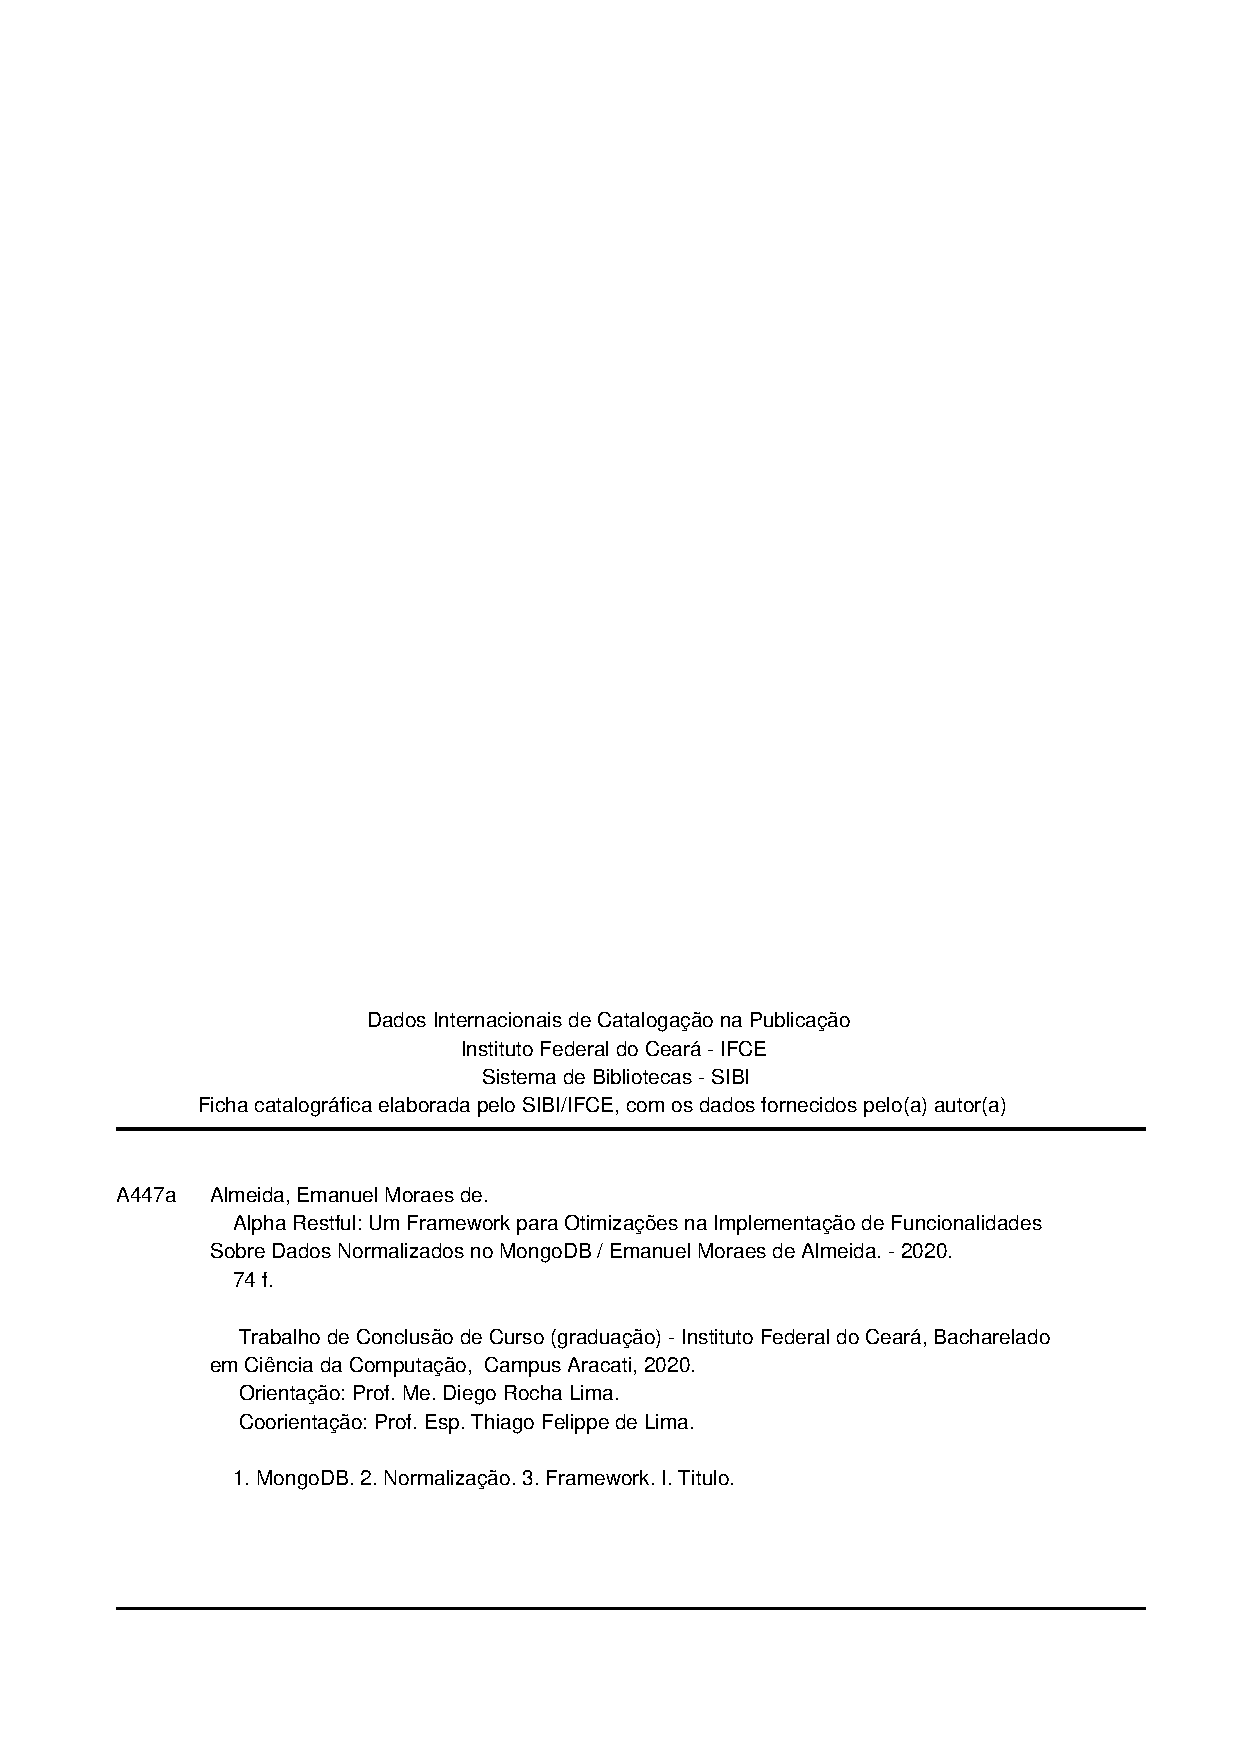
\includepdf[pages=-]{pdfs/fichacatalografica.pdf}
\begin{folhadeaprovacao}
\vfill
\begin{center}

{Emanuel Moraes de Almeida\\}
\vspace{1.5cm}
{\textsc{\uppercase{Desenvolvimento e Aplicação de um Framework para Otimizações na Implementação de Funcionalidades Sobre Dados Normalizados no \textit{MongoDB}}}\\}
\vspace{1.5cm}
\hspace{.45\linewidth}
\begin{minipage}{.50\linewidth}
Trabalho de Conclusão de Curso (TCC) apresentado ao curso de Bacharelado em Ciência da Computação do Instituto Federal de Educação, Ciência e Tecnologia do Ceará - IFCE - Campus Aracati, como requisito parcial para obtenção do Título de Bacharel em Ciência da Computação. 
\end{minipage}
\vspace{1.0 cm}

\end{center}

\noindent\\
{Aprovada em <data>}

\vspace{1.5 cm}
\begin{center}
{BANCA EXAMINADORA}
\assinatura{Prof. Me. Diego Rocha Lima (Orientador) \\Instituto Federal de Educação, Ciência e Tecnologia do Ceará}
\assinatura{Prof. Esp. Thiago Felippe de Lima Bandeira (Coorientador) \\Instituto Federal de Educação, Ciência e Tecnologia do Ceará}
\assinatura{Prof. Me. Érica de Lima Gallindo \\Instituto Federal de Educação, Ciência e Tecnologia do Ceará}
\assinatura{Prof. Me. Silas Santiago Lopes Pereira \\Instituto Federal de Educação, Ciência e Tecnologia do Ceará}

\end{center}
\end{folhadeaprovacao}
% \vfill
\begin{center}
{\textbf{DEDICATÓRIA}\\}
\end{center}

\noindent Aos meus pais.\\
\noindent Aos mestres.\\


% \vfill
\begin{center}
{\textbf{AGRADECIMENTOS}}
\end{center}

Agradecimentos aqui.



\vfill
\begin{center}
{\textbf{RESUMO}\\}
\end{center}
\noindent

Com a crescente demanda para armazenar uma quantidade cada vez maior de dados, os modelos de banco de dados tradicionais vêm demonstrando dificuldades no desenvolvimento de aplicações escaláveis, disponíveis e consistentes. Por isso, o modelo NoSQL tornou-se uma tecnologia emergente para suprir as deficiências do modelo relacional. Dentre os banco de dados NoSQL mais populares, encontra-se o \textit{MongoDB} que, apesar de facilitar o armazenamento de dados desnormalizados, muitas vezes não possui recursos simples e intuitivos para a manipulação de dados normalizados. Neste contexto, este trabalho apresenta um \textit{framework}, denominado \textit{Alpha Restful}, que propõe facilitar o desenvolvimento de funcionalidades sobre dados normalizados utilizando o \textit{MongoDB}. Como resultado, através de exemplos de código fonte, demonstrou-se de que forma o \textit{Alpha Restful} se sobressai em relação às alternativas apresentadas, comprovando a relevância deste estudo.

\vspace{\onelineskip}
 \noindent
 \textbf{Palavras-chaves}: \textit{MongoDB}; Normalização; \textit{Framework}.

\vfill
\begin{center}
{\textbf{ABSTRACT}\\}
\end{center}

\noindent

With the growing demand for storing an increasing amount of data, traditional database models have shown difficulties in developing scalable, available and consistent applications. For this reason, the NoSQL model has become an emerging technology to supply deficiencies in the relational model. Among the most popular NoSQL databases, MongoDB is found that, despite facilitating the storage of unnormalized data, it often does not have simple and intuitive resources for handling normalized data. In this context, this work presents a framework, called Alpha Restful, which proposes to facilitate the development of features on normalized data using MongoDB. As a result, through examples of source code, it was demonstrated how Alpha Restful stands out in relation to the alternatives presented, proving the relevance of this study.
 
 \vspace{\onelineskip}
    
 \noindent
 \textbf{Key words}: MongoDB; Normalization; \textit{Framework}; Alpha Restful.

% \vfill
\begin{center}
{\textbf{LISTA DE ILUSTRAÇÕES}}
\end{center}

\renewcommand\listfigurename{}
\listoffigures* % * indica que não aparecerá no sumário

\vfill
\begin{center}
{\textbf{LISTA DE TABELAS}}
\end{center}
\renewcommand\listtablename{}
\listoftables*
\vfill
\begin{center}
{\textbf{LISTA DE QUADROS}}
\end{center}

\renewcommand{\listofquadrosname}{}
\listofquadros*
\vfill
\begin{center}
{\textbf{LISTA DE EXEMPLOS}}
\end{center}

\renewcommand{\lstlistlistingname}{}
% \newlistof{lstlistoflistings}{lol}{\lstlistlistingname}
\lstlistoflistings*
\vfill
\begin{center}
{\textbf{LISTA DE ABREVIATURAS E SIGLAS}}
\end{center}
\vspace{0.5cm}

\begin{siglas}
% \item[IFCE] Instituto Federal de Educação, Ciência e Tecnologia do Ceará
% \item[TCC] Trabalho de Conclusão de Curso
\item[SQL] \textit{Structured Query Language}
\item[NoSQL] \textit{Not Only SQL}
\item[CRUD] \textit{Create, Read, Update e Delete}
\item[IoT] \textit{Internet of Things}
\item[JSON] \textit{JavaScript Object Notation}
\item[BJSON] \textit{Binary JSON}
\end{siglas}

\vfill
\begin{center}
{\textbf{SUMÁRIO}}
\end{center}

\renewcommand\contentsname{}
\tableofcontents*
\textual

%CAPITULOS
\chapter{INTRODUÇÃO}
\label{Introducao}

A grande demanda pela informatização de processos, que antes eram desenvolvidos completamente por humanos, tem sido bastante crescente. Isto vem estimulando a criação de novas ferramentas para facilitar o desenvolvimento de aplicações que automatizam tais processos. Para que tais aplicações possam se comunicar, torna-se necessário inseri-lo em uma rede local ou global de computadores. Dessa forma, o desenvolvimento \textit{Web} é usado para que a comunicação na rede do sistema desenvolvido possa acontecer.

%Uma aplicação pode ser desenvolvida em diversas plataformas. \hl{Uma das plataformas mais utilizadas atualmente é a web}, que permite a comunicação entre dispositivos localizados no mundo inteiro que se conectam a ela.

%%%%%
% A web pode realmente ser definida como uma plataforma?
%%%%%

%É comum uma aplicação web obedecer a um determinado padrão arquitetônico que irá definir regras para a organização dos seus pontos de acesso. Um dos padrões arquitetônicos mais utilizados é o REST.

\hl{Dentre as características mais comuns no desenvolvimento das mais diversas aplicações web}, estão a necessidade de armazenar, buscar, atualizar e remover dados, popularmente conhecido como CRUD (\textit{Create}, \textit{Read}, \textit{Update} e \textit{Delete}). Dependendo do propósito da aplicação desenvolvida, todas ou algumas dessas operações são utilizadas. \hl{Uma das abordagens mais antigas de armazenamento de dados é a utilização de arquivos de texto}, mas com o passar do tempo, \hl{gerenciar tais dados dessa maneira se tornou ineficiente}. Motivados por esta problemática, os Banco de Dados foram criados.

%%%%%
% Será que realmente deve ser afirmado que "Dentre as características mais comuns no desenvolvimento das mais diversas aplicações web"?

% Eu preciso provar que "Uma das abordagens mais antigas de armazenamento de dados é a utilização de arquivos de texto"?

% Eu preciso provar que "gerenciar tais dados dessa maneira se tornou ineficiente"?
%%%%%

% \hl{Um Banco de Dados é um sistema que possibilita o registro de dados seguindo uma determinada estrutura de armazenamento}

Assim como descrito por \cite{date2004introduccao}, um banco de dados é ``um sistema de armazenamento de dados baseado em computador; isto é, um sistema cujo objetivo global é registrar e manter informação''. \hl{Um SGBD (Sistema de Gerenciamento de Banco de Dados) é um software capaz de manipular um determinado banco de dados, disponibilizando para o usuário ferramentas de CRUD}. \hl{Um SGBD realiza todas as operações e tratamentos necessários, fornecendo um \textit{endpoint} de inserção de comandos para o gerenciamento mais simples, consistente e performático da manipulação de dados.}

%%%%%
% Buscar definição de banco de dados da literatura

% Buscar definição de SGBD da literatura

% Buscar na literatura as facilidades disponibilizadas por um SGBD
%%%%%

\hl{Vários tipos diferentes de Banco de Dados foram criados ao longo do tempo}, mas os Bancos de Dados \hl{atualmente mais utilizados pelas empresas seguem o modelo relacional}. \hl{Tal modelo define uma estrutura de dados normalizada baseado em tabelas que se relacionam entre si}. \hl{Tal modelo demonstrou-se consistente e performático, popularizando-se rapidamente}. \hl{A linguagem padrão utilizada por tais bancos é o SQL (Structured Query Languagem)}.

%%%%%
% Citar exemplos de tipos de bancos de dados

% Provar que o modelo mais utilizado atualmente é o modelo relacional

% Buscar definição de modelo relacional na literatura

% Fundamentar cientificamente que o modelo relacional "demonstrou-se consistente e performático, popularizando-se rapidamente"

% Quem definiu que o SQL é a linguagem padrão do modelo relacional? É necessário explicitar isso?
%%%%%

O modelo Relacional foi desenvolvido visando a imposição de alguns limites. Tais limites são definidos pelas regras de normalização \hl{e foram motivados para}:

%%%%%
% Justificar usando a literatura tais motivações
%%%%%

\begin{itemize}
	\item Otimizar a quantidade de dados armazenados;
	\item Otimizar a atualização de registros;
	\item Criar regras na própria estrutura de armazenamento, a fim de dificultar a inconsistência de dados.
\end{itemize}

\hl{Com o passar do tempo, os dispositivos começaram a aumentar sua capacidade de armazenamento drasticamente}. Tal avanço tecnológico estimulou a criação de aplicações que necessitam armazenar uma quantidade cada vez maior de dados. Mediante tal cenário, \hl{pôde-se observar} que os limites impostos pela normalização vêm demonstrando ser uma barreira tecnológica que dificulta a criação de aplicações altamente escaláveis, disponíveis e consistentes.

%%%%%
% Citar exemplos e estatísticas de como os dispositivos aumentaram sua capacidade de armazenamento

% Pôde-se observar como? Citar trabalhos relacionados que demonstre isso
%%%%%

Baseado nessa problemática, começaram a surgir novos modelos de armazenamento de dados, objetivando melhorar a performance de aplicações cujo o atendimento de suas exigências fosse muito caro, complexo ou inviável para o modelo de banco de dados Relacional.

\hl{Os bancos que estruturam seus dados usando abordagens não relacionais ou parcialmente relacionais são denominados de NoSQL (Not Only SQL)}. Vários tipos diferentes de banco de dados NoSQL foram surgindo, como por exemplo, os bancos baseados em células de \hl{tuplas, grafos, chave-valor e documento}.

%%%%%
% Buscar definição de NoSQL na literatura

% Referenciar trabalhos para esses tipos de NoSQL não abordados para demonstrar que eles existem
%%%%%

Atualmente, um dos banco de dados NoSQL \hl{mais utilizados é o \textit{MongoDB}}. Tal banco estrutura seus dados baseado em documentos. Esta abordagem quebra várias barreiras limitadas pelo modelo Relacional, permitindo que os dados sejam armazenados de maneira desnormalizada.

%%%%%
% Será que o MongoDB é um dos mais utilizados? Procurar referências na literatura para isso
%%%%%

A desnormalização permite uma maior flexibilização da estrutura de armazenamento, \hl{possibilitando a utilização de diversas técnicas específicas} para vários tipos de aplicações. Apesar dos benefícios da desnormalização, existem possíveis problemas que podem decorrer mediante seu uso.

%%%%%
% Que técnicas são permitidas pela flexibilização da estrutura de armazenamento? Onde na literatura isso é dito?
%%%%%

\hl{Os limites impostos pela normalização tentam garantir que um determinado valor somente precisará ser alterado em um único lugar}. Por causa desta característica, \hl{independente da complexidade do banco, a atualização de um valor, no geral, é bastante rápida}. Em contra partida, um banco desnormalizado não garante que um determinado valor estará em um único lugar, podendo exigir buscas possivelmente lentas para a localização de todos os locais onde o dado deve ser atualizado.

%%%%%
% Procurar na literatura que a normalização tende a "garantir que um determinado valor somente precisará ser alterado em um único lugar"

% Será mesmo que a atualização sempre tende a ser rápida no modelo relacional?
%%%%%

Por causa de tal problemática, aplicações que usam, por exemplo, o \textit{MongoDB}, podem sentir a necessidade de mesclar estratégias de normalização e desnormalização. Com o \textit{MongoDB}, os dados podem estar normalizados, parcialmente normalizados ou desnormalizados.

O \textit{MongoDB} foi projetado para que os dados possam estar desnormalizados e ele oferece \hl{um suporte muito bom para isto}, mas ele, atualmente, não oferece um suporte tão bom quanto em bancos relacionais para dados normalizados. Por causa disto, \hl{existem operações em dados normalizados que seriam mais simples de serem realizados usando a linguagem SQL, mas que se tornam mais difíceis de serem realizados no \textit{MongoDB}}. Dentro de um ambiente de desenvolvimento web com \textit{MongoDB}, tais problemáticas podem ser frequentemente encontradas.

%%%%%
% Justificar a afirmação do suporte ser muito bom para dados desnormalizados

% Justificar e demonstrar como e que operações são mais simples no SQL do que no MongoDB
%%%%%

O desenvolvimento de uma aplicação web com \textit{MongoDB} pode exigir um trabalho extra, em comparação com bancos relacionais, pois, as vezes, será necessário realizar uniões e buscas em dados normalizados ou parcialmente normalizados de forma não \hl{muito} intuitiva. Além disto, por causa da alta flexibilidade na estruturação dos dados, as diferentes formas como os dados podem ser armazenados exigem tratamentos \hl{muitos} distintos na hora de implementar funcionalidades comuns para o desenvolvimento web.

Dessa forma, se a estrutura dos dados mudar durante o desenvolvimento, as operações de busca e união precisarão ser alteradas. Ou seja, haverão mudanças em todas as funcionalidades que estiverem referenciando os dados reestruturados.

Além dos problemas decorrentes do uso do \textit{MongoDB}, uma aplicação web exige a implementação de um conjunto de funcionalidades que, apesar de serem comuns para este tipo de aplicação, podem exigir \hl{muito} trabalho para serem desenvolvidas.

Visando a resolução de tais problemas, este trabalho apresenta o desenvolvimento de um framework denominado \textit{Alpha Restful}, criado para desenvolver aplicações web com \textit{MongoDB} na linguagem \textit{ECMAScript} 6 (\textit{JavaScript}) e \textit{NodeJS} (no mínimo na versão 8).

\hl{Um framework é um conjunto de códigos fonte que oferece camadas de abstração para facilitar o desenvolvimento de um conjunto de funcionalidades disponibilizadas por ele}.

%%%%%
% Buscar na literatura a definição de framework
%%%%%

O \textit{Alpha Restful} abstrai a implementação de diversas funcionalidades que precisariam ser desenvolvidas manualmente. O desenvolvimento feito usando tal framework torna-se mais simples, pois ele obtém informações sobre a forma como os dados estão armazenados. Essas informações são utilizadas para que diversas funcionalidades sejam abstraídas em implementações mais simples e direcionadas ao que realmente se deseja fazer. 

%O \textit{Alpha Restful} pode ser dividido em 3 camadas de abstração, que serão explicadas posteriormente.

%A primeira camada é a de modelagem. Nela o desenvolvedor irá descrever a forma como os dados serão armazenados. Nesta camada será possível criar um padrão a ser seguido na hora de salvar os dados. Tal padrão irá definir quais dados estarão normalizados, desnormalizados ou parcialmente normalizados. Nesta camada, será possível informar comportamentos específicos para cada valor armazenado.

%Nesta etapa o framework irá gerar metadados (conjunto de dados que descrevem informações sobre a forma como os dados estão estruturados). Tais metadados serão utilizados pelas camadas seguintes a fim de automatizar a implementação de várias funcionalidades. Com os dados da modelagem (descrição feita pelo usuário) e com os metadados (dados gerados pelo \textit{Alpha Restful}), diversas funcionalidades serão implementadas pelo próprio framework, exigindo apenas que o usuário informe informações descritivas na hora de desenvolver tais funções. Por causa de tal abstração, pesquisas podem ser realizadas da mesma maneira, independente dos dados estarem normalizados, desnormalizados ou parcialmente normalizados.

%A segunda camada é a de CRUD automático. Nela o framework poderá criar (bastando apenas a habilitação desta opção) automaticamente todo o CRUD da aplicação. Operações de registro, remoção, atualização e busca serão criados automaticamente, sem que nenhuma codificação seja necessária.

%Nesta etapa, o framework irá implementar uma funcionalidade de busca padrão. Nela, serão utilizados os dados e metadados da modelagem para prever uma enorme quantidade de possibilidades de pesquisas possíveis. A customização desta camada é limitada em um conjunto enumerável de opções. Para aplicações simples, o \textit{Alpha Restful} exigirá apenas a definição da modelagem e o sistema estará pronto.

%Ainda nesta camada, alguns comportamentos padrão serão automaticamente executados, tendo como base as informações definidas na primeira camada. Um destes comportamentos é a relação de dependência entre os documentos. Isto permite que entidades sejam removidas em cascata, ou que sejam desreferenciadas (uma determinada chave estrangeira seja removida de uma entidade relacionada) ou ainda que sejam impedidas de serem removidas tendo como base a remoção de uma outra entidade relacionada.

%A segunda camada é muito poderosa e implementa diversas funcionalidades automaticamente tendo como base a modelagem definida pelo usuário. As customizações podem ser realizadas na modelagem dos dados, mas o número de customizações são finitas e enumeráveis, apesar de bastante poderosas e poderem ser usadas recursivamente.

%Caso a segunda camada não seja o suficiente, é disponibilizado uma terceira camada de abstração. Nela, um conjunto de funcionalidades bastante comuns em aplicações web REST podem ser definidas. Nesta camada, várias funcionalidades poderão ser feitas baseando-se em um padrão descritivo, ou seja, ao invés de o desenvolvedor precisar chamar as funções disponibilizadas pelo \textit{MongoDB}, o próprio framework se encarregará de realizar esta chamada. A única coisa que o desenvolvedor precisará fazer é disponibilizar um objeto que contém a descrição do que ele deseja que seja feito. Esta descrição é algo bem enxuto, tendo em vista que o \textit{Alpha Restful} já conhece a forma pela qual os dados estão estruturados e já possui diversos dados e metadados sobre comportamentos específicos de cada valor salvo definido na camada de modelagem. As pesquisas implementadas nesta camada, por causa de sua abstração, são realizados da mesma maneira, independente dos dados estarem normalizados, desnormalizados ou parcialmente normalizados.

\section{Objetivos}
\subsection{Objetivo Geral}
\subsection{Objetivos Específicos}

\section{Organização do Trabalho}
\chapter{FUNDAMENTAÇÃO TEÓRICA}
\label{FundamentacaoTeorica}

\section{Modelo de Banco de Dados Relacional}

O modelo relacional surgiu por volta dos anos de 1970, com base no modelo proposto por \citeonline{codd1970relational}. Através deste modelo, ``os dados são armazenados com um forte grau de independência, desacoplando a lógica, da representação dos dados'' \cite{davoudian2018survey}. Na representação relacional, os dados são normalizados e as diversas relações (tabelas) podem referenciar os dados contidos em outras tabelas.

Assim como explicado por \citeonline{date2004introduccao}, cada linha de uma tabela (tupla) deve representar a abstração de um objeto do sistema, sendo que cada célula é uma característica (atributo) do objeto representado. Cada tupla deve possuir pelo menos uma célula como identificador único (chave primária) que irá representar todos os dados contido na linha a qual ela está contida. A chave primária é um valor único para a tabela, geralmente representado com um tipo numérico. Tal chave pode ser armazenada em outras tabelas por meio do uso de chaves estrangeiras. Uma chave estrangeira é uma (ou mais de uma) chave primária de outra relação. Armazenar tal chave simboliza que os dados representados por ela estão contidos dentro da tabela.

Como exemplo, pode-se abstrair um sistema que precisa armazenar várias pessoas (na qual cada uma possui um nome e uma idade) e várias casas (que possui uma rua e número). A tabela \ref{tab: pessoa} apresenta como as pessoas podem estar representadas no banco de dados.

%%%%% REMOVIDO %%%%%
% Caso seja necessário armazenar os dados contidos em uma tupla de outra relação, basta, em alguma célula da tupla, armazenar uma chave estrangeira (chave primária de uma tupla de outra relação) de outra tabela. Ao armazenar como chave estrangeira a chave primária de outra tabela, é gerado um link lógico, simbolizando que todos os dados representados por esta chave estrangeira também estão contidos dentro desta mesma tupla.
%%%%% REMOVIDO %%%%%

%IMPORTANTE
%Os exemplos precisam ser referenciados

\begin{longtable}[]{@{}lll@{}}
\caption{Exemplo de relação de pessoas \label{tab: pessoa}}\tabularnewline
\toprule
Chave Primária & Nome & Idade \tabularnewline
\midrule
\endfirsthead
\toprule
Chave Primária & Nome & Idade\tabularnewline
\midrule
\endhead
1 & Emanuel & 21\tabularnewline
2 & Eduardo & 40\tabularnewline
\bottomrule
% \caption*{Fonte: O autor (2020)}
\end{longtable}

%%%%% REMOVIDO %%%%%
% \begin{table}[h]
%     \centering
%     \begin{tabular}{|c|c|c|}
%         \hline
%         \rowcolor[HTML]{FFAC71} 
%         \multicolumn{3}{|c|}{\cellcolor[HTML]{FFAC71}pessoa}                                                                                          \\ \hline
%         \rowcolor[HTML]{9698ED} 
%         {\color[HTML]{000000} \begin{tabular}[c]{@{}c@{}}Chave \\ Primária\end{tabular}} & {\color[HTML]{000000} Nome} & {\color[HTML]{000000} Idade} \\ \hline
%         1                                                                                & Emanuel                     & 21                           \\ \hline
%         2                                                                                & Eduardo                     & 40                           \\ \hline
%     \end{tabular}
%     \label{tab-ex1: pessoa}
%     \caption{Relação de pessoas}
% \end{table}

% \begin{table}[h]
%     \centering{
%         \begin{tabular}{|c|c|c|}
%             \hline
%             \rowcolor[HTML]{67FD9A} 
%             \multicolumn{3}{|c|}{\cellcolor[HTML]{67FD9A}casa}                                                                                            \\ \hline
%             \rowcolor[HTML]{9698ED} 
%             {\color[HTML]{000000} \begin{tabular}[c]{@{}c@{}}Chave \\ Primária\end{tabular}} & {\color[HTML]{000000} Rua} & {\color[HTML]{000000} Número} \\ \hline
%             10                                                                               & Rua Castelo Branco         & 1B                            \\ \hline
%             20                                                                               & Rua Pompel                 & 1089                          \\ \hline
%         \end{tabular}
%     }
% \end{table}
%%%%% REMOVIDO %%%%%

Continuando com o exemplo, naturalmente, no desenvolvimento de um sistema, as entidades se relacionam entre si. Neste caso, uma pessoa pode possuir várias casas, mas uma casa possui apenas uma pessoa como dono. Para representar essa relação, precisa-se definir quem será o dono da relação, ou seja, quem irá receber a chave primária da outra entidade através de uma chave estrangeira. Sempre deverá existir apenas  um dono da relação, ou seja, a chave estrangeira desta relação deverá estar em apenas uma tabela.
    
Como uma pessoa pode possuir várias casas, o dono da relação deve ser a casa, caso contrário a tupla de uma pessoa teria que ser duplicada (a menos que uma terceira tabela seja criada). Para representar as casas neste contexto, pode-se modelar os dados assim como demonstrado na tabela \ref{tab: casa}. Nela, pode-se observar que a pessoa Emanuel possui as duas casas armazenados no banco de dados, enquanto o Eduardo não possui nenhuma casa.

\begin{longtable}[]{@{}llll@{}}
\caption{Exemplo de relação de casas \label{tab: casa}}\tabularnewline
\toprule
Chave Primária & Rua & Número & Chave Estrangeira de Pessoa\tabularnewline
\midrule
\endfirsthead
\toprule
Chave Primária & Rua & Número & Chave Estrangeira de Pessoa\tabularnewline
\midrule
\endhead
10 & Rua Castelo Branco & 1B & 1\tabularnewline
20 & Rua Pompel & 1089 & 1\tabularnewline
\bottomrule
% \caption*{Fonte: O autor (2020)}
\end{longtable}

%%%%% REMOVIDO %%%%%
% \begin{table}[h]
%     \centering
%     \begin{tabular}{|c|c|c|c|}
%         \hline
%         \rowcolor[HTML]{67FD9A} 
%         \multicolumn{4}{|c|}{\cellcolor[HTML]{67FD9A}casa}                                                                                                                                                                        \\ \hline
%         \rowcolor[HTML]{9698ED} 
%         {\color[HTML]{000000} \begin{tabular}[c]{@{}c@{}}Chave \\ Primária\end{tabular}} & {\color[HTML]{000000} Rua} & {\color[HTML]{000000} Número} & \begin{tabular}[c]{@{}c@{}}Chave \\ Estrangeira \\ de pessoa\end{tabular} \\ \hline
%         10                                                                               & Rua Castelo Branco         & 1B                            & 1                                                                         \\ \hline
%         20                                                                               & Rua Pompel                 & 1089                          & 1                                                                         \\ \hline
%     \end{tabular}
%     \label{tab-ex1: casa}
%     \caption{Relação de casas}
% \end{table}
%%%%% REMOVIDO %%%%%

\subsection{Normalização}

O modelo relacional possui algumas regras que o desenvolvedor observa ao modelar as estruturas das relações de seu banco. Dentre estas regras estão contidas as regras de normalização. ``O objetivo da normalização é evitar os problemas de banco de dados, bem como eliminar a `mistura de assuntos' e as correspondentes redundâncias desnecessárias de dados'' \cite{machado2020banco}. Com a redução dessas ``redundâncias desnecessárias'', uma otimização da quantidade de dados é alcançada. \citeonline{machado2020banco} descreve 5 formas normais. Destas, apenas as 3 primeiras serão explicitadas a seguir, por terem impacto mais significante para os propósitos deste trabalho.

%%%%% DÚVIDAS %%%%%
% As regras de nornalização realmente devem ser seguidas em todas as circunstâncias?
% R - creio que são questões organizacionais e que facilitam as consultas
%%%%% DÚVIDAS %%%%%

%%%%% PENDÊNCIAS %%%%%
% Justificar através de citações o parâgrafo anterior
%%%%% PENDÊNCIAS %%%%%

\subsubsection{Primeira Forma Normal}
    
Como visto anteriormente, uma tupla representa um objeto da entidade representada pela relação a qual a tupla pertence. Tendo esse princípio como base, como é possível representar a situação de uma casa possuir vários donos e ao mesmo tempo uma pessoa possuir várias casas?
    
O princípio da primeira forma normal define que nunca deve-se duplicar colunas em várias linhas, garantindo que duas ou mais tuplas nunca representem o mesmo objeto. Para manter este princípio e ainda realizar um relacionamento de muitos para muitos (uma pessoa tem muitas casas e uma casa tem muitas pessoas), torna-se necessário a criação de uma tabela auxiliar para representar o relacionamento de pessoa com casa. A tabela \ref{tab: relacionamento-pessoa-casa} exemplifica a criação de uma tabela auxiliar, na qual a pessoa ``Emanuel'' possui as duas casas e o ``Eduardo'' possui a casa de número 1B.

\begin{longtable}[]{@{}lll@{}}
\caption{Exemplo de tabela auxiliar \label{tab: relacionamento-pessoa-casa}}\tabularnewline
\toprule
Chave Primária & Chave Estrangeira de Pessoa & Chave Estrangeira de Casa\tabularnewline
\midrule
\endfirsthead
\toprule
Chave Primária & Chave Estrangeira de Pessoa & Chave Estrangeira de Casa\tabularnewline
\midrule
\endhead
100 & 1 & 10\tabularnewline
200 & 1 & 20\tabularnewline
300 & 2 & 10\tabularnewline
\bottomrule
% \caption*{Fonte: O autor (2020)}
\end{longtable}

%%%%% REMOVIDO %%%%%
% \begin{longtable}[]{@{}llcl@{}}
% \caption{Exemplo de relação de pessoas \label{tab-ex2: pessoa}}\tabularnewline
% \toprule
% Chave Primária & Nome & Idade \tabularnewline
% \midrule
% \endfirsthead
% \toprule
% Chave Primária & Nome & Idade\tabularnewline
% \midrule
% \endhead
% 1 & Emanuel & 21\tabularnewline
% 2 & Eduardo & 40\tabularnewline
% \bottomrule
% \caption*{Fonte: O autor (2020)}
% \end{longtable}

% \begin{longtable}[]{@{}llcl@{}}
% \caption{Exemplo de relação de casas \label{tab-ex2: casa}}\tabularnewline
% \toprule
% Chave Primária & Rua & Número & Chave Estrangeira de pessoa\tabularnewline
% \midrule
% \endfirsthead
% \toprule
% Chave Primária & Rua & Número & Chave Estrangeira de pessoa\tabularnewline
% \midrule
% \endhead
% 10 & Rua Castelo Branco & 1B & 1\tabularnewline
% 20 & Rua Pompel & 1089 & 1\tabularnewline
% \bottomrule
% \caption*{Fonte: O autor (2020)}
% \end{longtable}

% \begin{table}[h]
%         \centering
%         \begin{tabular}{|c|c|c|}
%             \hline
%             \rowcolor[HTML]{FFAC71} 
%             \multicolumn{3}{|c|}{\cellcolor[HTML]{FFAC71}pessoa}                                                                                          \\ \hline
%             \rowcolor[HTML]{9698ED} 
%             {\color[HTML]{000000} \begin{tabular}[c]{@{}c@{}}Chave \\ Primária\end{tabular}} & {\color[HTML]{000000} Nome} & {\color[HTML]{000000} Idade} \\ \hline
%             1                                                                                & Emanuel                     & 21                           \\ \hline
%             2                                                                                & Eduardo                     & 40                           \\ \hline
%         \end{tabular}
% \end{table}
    
% \begin{table}[h]
%         \centering
%         \begin{tabular}{|c|c|c|}
%             \hline
%             \rowcolor[HTML]{FCFF2F} 
%             \multicolumn{3}{|c|}{\cellcolor[HTML]{FCFF2F}Relacionamentopessoacasa}                                                                                                                                                                                                                                   \\ \hline
%             \rowcolor[HTML]{9698ED} 
%             {\color[HTML]{000000} \begin{tabular}[c]{@{}c@{}}Chave \\ Primária do\\ Relacionamento\end{tabular}} & {\color[HTML]{000000} \begin{tabular}[c]{@{}c@{}}Chave \\ Estrangeira \\ de pessoa\end{tabular}} & {\color[HTML]{000000} \begin{tabular}[c]{@{}c@{}}Chave \\ Estrangeira \\ de casa\end{tabular}} \\ \hline
%             100                                                                                                    & 1                                                                                                & 10                                                                                             \\ \hline
%             200                                                                                                    & 1                                                                                                & 20                                                                                             \\ \hline
%             300                                                                                                    & 2                                                                                                & 10                                                                                             \\ \hline
%         \end{tabular}
% \end{table}
    
% \begin{table}[h]
%         \centering
%         \begin{tabular}{|c|c|c|}
%             \hline
%             \rowcolor[HTML]{67FD9A} 
%             \multicolumn{3}{|c|}{\cellcolor[HTML]{67FD9A}casa}                                                                                            \\ \hline
%             \rowcolor[HTML]{9698ED} 
%             {\color[HTML]{000000} \begin{tabular}[c]{@{}c@{}}Chave \\ Primária\end{tabular}} & {\color[HTML]{000000} Rua} & {\color[HTML]{000000} Número} \\ \hline
%             10                                                                               & Rua Castelo Branco         & 1B                            \\ \hline
%             20                                                                               & Rua Pompel                 & 1089                          \\ \hline
%         \end{tabular}
% \end{table}
%%%%% REMOVIDO %%%%%
    
\subsubsection{Segunda Forma Normal}
    
A segunda forma normal especifica que todos os dados de uma tupla devem ser representados por toda a sua chave primária e jamais por apenas parte dela. Como exemplo disto pode-se afirmar que uma casa jamais poderia ser armazenado dentro da mesma tupla de uma pessoa, mesmo em um relacionamento um para um (Uma pessoa para uma casa e uma casa para uma pessoa). Isto ocorre pois os dados de uma casa são independentes dos dados de uma pessoa e a chave primária de uma pessoa não poderia representar também os dados de uma casa.
    
Uma chave primária também pode ser composta por várias células, mas todos os dados da tupla devem depender de todas as células da chave primária. Caso exista algum dado que dependa apenas de parte da chave primária, uma nova tabela deve ser criada. Uma tabela somente está na segunda forma normal se também estiver na primeira forma normal.
    
\subsubsection{Terceira Forma Normal}
    
Continuando o exemplo, pode-se imaginar que devem existir atributos no relacionamento entre pessoa e casa, indicando o valor mensal que a pessoa deve pagar como aluguel pela casa, a quantidade de meses a pagar o aluguel e o total a pagar até o fim do contrato. Para isso, poderíamos adicionar tais atributos na tabela de relacionamento de pessoa com casa, assim como descrito na tabela \ref{tab: atributos-relacionamento}. Nesta, a pessoa de nome ``Emanuel'' paga 200 reais pela casa de número 1B com contrato válido por 12 meses e paga 400 reais pela casa de número 1089 com contrato válido por 24 meses. O Eduardo paga 300 reais pela casa de número 1B com contrato válido por 8 meses.

\begin{longtable}[]{@{}llllll@{}}
\caption{Exemplo Atributos no Relacionamento \label{tab: atributos-relacionamento}}\tabularnewline
\toprule
Chave Primária & Pessoa & Casa & Valor Mensal & Quantidade de Meses & Total\tabularnewline
\midrule
\endfirsthead
\toprule
Chave Primária & Pessoa & Casa & Valor Mensal & Quantidade de Meses & Total\tabularnewline
\midrule
\endhead
100 & 1 & 10 & 200 & 12 & 2400\tabularnewline
200 & 1 & 20 & 400 & 24 & 9600\tabularnewline
300 & 2 & 10 & 300 & 8  & 2400\tabularnewline
\bottomrule
% \caption*{Fonte: O autor (2020)}
\end{longtable}

%%%%% REMOVIDO %%%%%
% \begin{table}[h]
%     \centering
%     \begin{tabular}{|c|c|c|c|c|c|}
%         \hline
%         \rowcolor[HTML]{FCFF2F} 
%         \multicolumn{6}{|c|}{\cellcolor[HTML]{FCFF2F}Relacionamentopessoacasa}                                                                                                                                                                                                                                                                                                                                                                                                                      \\ \hline
%         \rowcolor[HTML]{9698ED} 
%         {\color[HTML]{000000} \begin{tabular}[c]{@{}c@{}}Chave \\ Primária do\\ Relacionamento\end{tabular}} & {\color[HTML]{000000} \begin{tabular}[c]{@{}c@{}}Chave \\ Estrangeira \\ de pessoa\end{tabular}} & {\color[HTML]{000000} \begin{tabular}[c]{@{}c@{}}Chave \\ Estrangeira \\ de casa\end{tabular}} & \begin{tabular}[c]{@{}c@{}}Valor\\ Mensal\end{tabular} & \begin{tabular}[c]{@{}c@{}}Quantidade\\ de Meses\end{tabular} & \begin{tabular}[c]{@{}c@{}}Total a\\ Pagar\end{tabular} \\ \hline
%         100                                                                                                    & 1                                                                                                & 10                                                                                             & 200                                                    & 12                                                            & 2400                                                    \\ \hline
%         200                                                                                                    & 1                                                                                                & 20                                                                                             & 400                                                    & 24                                                            & 9600                                                    \\ \hline
%         300                                                                                                    & 2                                                                                                & 10                                                                                             & 300                                                    & 8                                                             & 2400                                                    \\ \hline
%     \end{tabular}
% \end{table}
%%%%% REMOVIDO %%%%%
    
Para este caso, a relação \ref{tab: atributos-relacionamento} não está na terceira forma normal, pois o atributo \textit{Total} é dependente do \textit{Valor Mensal} e da \textit{Quantidade de Meses}. O \textit{Total} pode ser obtido através de uma busca no banco de dados, realizando uma simples multiplicação do \textit{Valor Mensal} e da \textit{Quantidade de Meses}. Para que esta relação fique de acordo com a Terceira Forma Normal é necessário remover a última coluna, assim como apresentado na tabela \ref{tab: total-a-pagar-removido}.

\begin{longtable}[]{@{}lllll@{}}
\caption{Relacionamento sem o ``Total'' \label{tab: total-a-pagar-removido}}\tabularnewline
\toprule
Chave Primária & Pessoa & Casa & Valor Mensal & Quantidade de Meses\tabularnewline
\midrule
\endfirsthead
\toprule
Chave Primária & Pessoa & Casa & Valor Mensal & Quantidade de Meses\tabularnewline
\midrule
\endhead
100 & 1 & 10 & 200 & 12\tabularnewline
200 & 1 & 20 & 400 & 24\tabularnewline
300 & 2 & 10 & 300 & 8\tabularnewline
\bottomrule
% \caption*{Fonte: O autor (2020)}
\end{longtable}

%%%%% REMOVIDO %%%%%
% \begin{table}[h]
%     \centering
%     \begin{tabular}{|c|c|c|c|c|}
%         \hline
%         \rowcolor[HTML]{FCFF2F} 
%         \multicolumn{5}{|c|}{\cellcolor[HTML]{FCFF2F}Relacionamentopessoacasa}                                                                                                                                                                                                                                                                                                                                                            \\ \hline
%         \rowcolor[HTML]{9698ED} 
%         {\color[HTML]{000000} \begin{tabular}[c]{@{}c@{}}Chave \\ Primária do\\ Relacionamento\end{tabular}} & {\color[HTML]{000000} \begin{tabular}[c]{@{}c@{}}Chave \\ Estrangeira \\ de pessoa\end{tabular}} & {\color[HTML]{000000} \begin{tabular}[c]{@{}c@{}}Chave \\ Estrangeira \\ de casa\end{tabular}} & \begin{tabular}[c]{@{}c@{}}Valor\\ Mensal\end{tabular} & \begin{tabular}[c]{@{}c@{}}Quantidade\\ de Meses\end{tabular} \\ \hline
%         1                                                                                                    & 1                                                                                                & 10                                                                                             & 200                                                    & 12                                                            \\ \hline
%         2                                                                                                    & 1                                                                                                & 20                                                                                             & 400                                                    & 24                                                            \\ \hline
%         3                                                                                                    & 2                                                                                                & 10                                                                                             & 300                                                    & 8                                                             \\ \hline
%     \end{tabular}
% \end{table}
%%%%% REMOVIDO %%%%%
    
A terceira forma normal especifica que não deve existir uma célula que dependa de outras células. Cada valor deverá ser o mais independente possível dos outros valores. Para que uma relação esteja na terceira forma normal, também torna-se necessário que esteja na segunda forma normal.

\subsection{Junção de Tabelas\label{subsection: juncao-tabelas}}
    
Assim como descrito por \citeonline{machado2020banco}, existem situações onde as tabelas precisam ser unidas em uma única tabela, para que os dados contidos em diversas relações, que são necessários à consulta formulada, possam ser acessados. Como exemplo disto, pode-se unir as tabelas \ref{tab: pessoa}, \ref{tab: casa} e \ref{tab: total-a-pagar-removido}, para a pessoa de nome \textit{Emanuel}. No exemplo \ref{lst: uniao-tabelas-sql} encontra-se uma codificação SQL para a união de tabelas para o contexto apresentado. A seguir, na tabela \ref{tab: juncao-de-tabelas-para-emanuel} apresenta-se o resultado de tal codificação.

% \newpage

\begin{lstlisting}[language=SQL, caption={União de Tabelas com SQL\label{lst: uniao-tabelas-sql}}]
    SELECT p.id as Pessoa, p.nome as Nome, p.idade as Idade, rpc.valor_mensal as ValorMensal, rpc.quantidade_meses as Meses, c.id as Casa, c.rua as Rua, c.numero as Numero
    FROM pessoa p JOIN
        Relacionamentopessoacasa rpc ON p.id = rpc.pessoa_id JOIN
        casa c ON rpc.casa_id = c.id
    WHERE p.nome = "Emanuel"
\end{lstlisting}

\newpage

\begin{longtable}[]{@{}llllllll@{}}
\caption{Junção de Tabelas Para Emanuel \label{tab: juncao-de-tabelas-para-emanuel}}\tabularnewline
\toprule
\footnotesize{Pessoa} & \footnotesize{Nome} & \footnotesize{Idade} & \footnotesize{ValorMensal} & \footnotesize{Meses} & \footnotesize{Casa} & \footnotesize{Rua} & \footnotesize{Numero}\tabularnewline
\midrule
\endfirsthead
\toprule
\footnotesize{Pessoa} & \footnotesize{Nome} & \footnotesize{Idade} & \footnotesize{ValorMensal} & \footnotesize{Meses} & \footnotesize{Casa} & \footnotesize{Rua} & \footnotesize{Numero}\tabularnewline
\midrule
\endhead
\footnotesize{1} & \footnotesize{Emanuel} & \footnotesize{21} & \footnotesize{200} & \footnotesize{12} & \footnotesize{10} & \footnotesize{Rua Castelo Branco} & \footnotesize{1B}\tabularnewline
\footnotesize{1} & \footnotesize{Emanuel} & \footnotesize{21} & \footnotesize{400} & \footnotesize{24} & \footnotesize{20} & \footnotesize{Rua Pompel} & \footnotesize{1089}\tabularnewline
\bottomrule
% \caption*{Fonte: O autor (2020)}
\end{longtable}

%%%%% REMOVIDO %%%%%
%     \begin{table}[h]
%         \centering
%         \resizebox{\textwidth}{!}{%
%             \begin{tabular}{|c|c|c|c|c|c|c|c|c|c|c|}
%                 \hline
%                 \rowcolor[HTML]{38FFF8} 
%                 \multicolumn{11}{|c|}{\cellcolor[HTML]{38FFF8}Junção das Três Tabelas}                                                                                                                                                                                                                                                                                                                                                                                                                                                                                                                                                        \\ \hline
%                 \rowcolor[HTML]{9698ED} 
%                 \begin{tabular}[c]{@{}c@{}}Chave\\ Primária\\ de pessoa\end{tabular} & Nome    & Idade & {\color[HTML]{000000} \begin{tabular}[c]{@{}c@{}}Chave \\ Primária do\\ Relacionamento\end{tabular}} & {\color[HTML]{000000} \begin{tabular}[c]{@{}c@{}}Chave \\ Estrangeira \\ de pessoa\end{tabular}} & {\color[HTML]{000000} \begin{tabular}[c]{@{}c@{}}Chave \\ Estrangeira \\ de casa\end{tabular}} & \begin{tabular}[c]{@{}c@{}}Valor\\ Mensal\end{tabular} & \begin{tabular}[c]{@{}c@{}}Quantidade\\ de Meses\end{tabular} & \begin{tabular}[c]{@{}c@{}}Chave\\ Primária\\ de casa\end{tabular} & Rua                & Número \\ \hline
%                 1                                                                    & Emanuel & 21    & 100                                                                                                    & 1                                                                                                & 10                                                                                             & 200                                                    & 12                                                            & 10                                                                 & Rua Castelo Branco & 1B     \\ \hline
%                 1                                                                    & Emanuel & 21    & 200                                                                                                    & 1                                                                                                & 20                                                                                             & 400                                                    & 24                                                             & 20                                                                 & Rua Pompel & 1089     \\ \hline
%             \end{tabular}%
%         }
%     \end{table}
    
% Neste caso, algumas colunas do relacionamento de pessoa com casa são desnecessárias e no comando de junção das tabelas pode-se omití-las. Neste caso a tabela de junção seria algo como:
    
%     \begin{table}[h]
%         \centering
%         \resizebox{\textwidth}{!}{%
%             \begin{tabular}{|c|c|c|c|c|c|c|c|}
%                 \hline
%                 \rowcolor[HTML]{38FFF8} 
%                 \multicolumn{8}{|c|}{\cellcolor[HTML]{38FFF8}Junção das Três Tabelas}                                                                                                                                                                                                                                              \\ \hline
%                 \rowcolor[HTML]{9698ED} 
%                 \begin{tabular}[c]{@{}c@{}}Chave\\ Primária\\ de pessoa\end{tabular} & Nome    & Idade & \begin{tabular}[c]{@{}c@{}}Valor\\ Mensal\end{tabular} & \begin{tabular}[c]{@{}c@{}}Quantidade\\ de Meses\end{tabular} & \begin{tabular}[c]{@{}c@{}}Chave\\ Primária\\ de casa\end{tabular} & Rua                & Número \\ \hline
%                 1                                                                    & Emanuel & 21    & 200                                                    & 12                                                            & 10                                                                 & Rua Castelo Branco & 1B     \\ \hline
%                 1                                                                    & Emanuel & 21    & 400                                                    & 24                                                             & 20                                                                 & Rua Pompel & 1089     \\ \hline
%             \end{tabular}%
%         }
%     \end{table}
%%%%% REMOVIDO %%%%%

Quando há a separação dos dados, a atualização destes tendem a garantir uma maior consistência, além de tentar garantir que os valores precisarão ser atualizados em um único local. Mas em buscas no banco de dados, as junções de tabelas são, muitas vezes, inevitáveis.

%%%%% PENDÊNCIAS %%%%%
% Referenciar trabalhos que demonstrem que a separação dos dados tem o proposito apresentado no parágrafo anterior
% R - nesse caso também não precisa referenciar, pois vc ta fazendo uma constatação de quem programa
%%%%% PENDÊNCIAS %%%%%
    
Em um sistema complexo, com uma grande quantidade de dados e relações, cada tabela poderá conter milhares ou até milhões de linhas. Uma operação de junção, envolvendo muitos dados, pode ser lento demais para os requisitos da aplicação. Existem algumas técnicas e estratégias para deixar essas consultas mais rápidas, como, por exemplo, o uso de índices. Mas mesmo com essas estratégias, haverá aplicações na qual a exigência de alta performance, escalabilidade, disponibilidade e consistência tornará inviável ou altamente caro escalar uma aplicação utilizando o modelo relacional.

%%%%% PENDÊNCIAS %%%%%
% Referenciar na literatura tais técnicas e estratégias
% R - Nesse caso se encontrar algum trabalho seria bom, mas ainda assim não é obrigatório.
%%%%% PENDÊNCIAS %%%%%

\subsection{Vantagens do Modelo relacional}
    
\begin{itemize}
    \item O modelo relacional já está bem solidificado no mercado, possuindo várias ferramentas e \textit{frameworks} para facilitar o desenvolvimento dos mais diversos tipos de aplicações;
        
    \item Pelo fato do modelo relacional forçar a separação e normalização dos dados, torna-se mais difícil que erros humanos ou de desenvolvimento venham a fazer os dados perderem sua consistência;
        
%    \item A normalização dos dados proporciona que os dados possam ser
%         inseridos/atualizados sem que o usuário/desenvolvedor tenha a responsabilidade de 
%         fazer diversas verificações físicas/lógicas na própria estrutura de armazenamento de
%         dados;
        
%    \item Uma modelagem de dados mal planejada possui menos chances de causar grandes
%         danos a consistência dos dados por causa da normalização;
        
    \item A normalização, por causa de seu princípio de não repetir dados em várias tabelas, tende a diminuir o espaço necessário para armazenar os dados, além de a atualização de registros, no geral, ocorrer em apenas um local.
\end{itemize}
    
\subsection{Desvantagens do Modelo relacional}

%%%%% DÚVIDAS %%%%%
% Precisa justificar tais desvantagens por meio de citações às referências bibliográficas?
%%%%% DÚVIDAS %%%%%
    
\begin{itemize}
    \item Os recursos de modelagem são muito limitados;
        
    \item A construção de objetos por meio de operações de junção, muitas vezes, são caras;
        
    \item O modelo relacional revelou deficiências no armazenamento e consulta de um grande volume de dados;
        
    \item Diversas aplicações com altos requisitos de escalabilidade, disponibilidade e consistência se tornam caras ou inviáveis no modelo relacional;
        
    \item As aplicações precisam se adaptar ao modelo relacional. Mesmo que uma aplicação possa ter uma parte dos dados não normalizados, sem prejudicar a consistência (por causa de alguma regra de negócio), o modelo relacional exige a normalização em vários casos, para um bom funcionamento das consultas.
\end{itemize}

\section{Modelo de Banco de Dados NoSQL com \textit{MongoDB}}

%%%%% REMOVIDO %%%%%
% Desde o início dos anos 2000, os avanços na tecnologia web, resultaram na explosão repentina de dados estruturados, semi-estruturados e não estruturados por aplicativos de escopo global. Tais aplicações geralmente exigem uma escalabilidade horizontal, adaptar-se às enormes quantidades de dados e à taxa crescente de processamento de consultas \citeonline{davoudian2018survey}.

% A alta disponibilidade, a baixa tolerância a falhas para responder aos clientes, confiabilidade de transações, o suporte a dados altamente consistentes e a manutenção de \textit{schemas} de banco de dados com baixo custo de evolução do sistema são requisitos que se tornam muitos difíceis ou inatingíveis nos sistemas tradicionais de banco de dados relacional \citeonline{davoudian2018survey}.Além desse motivo, a ampliação de sistemas exige uma movimentação de servidores autônomos com hardware aprimorados, sendo um processo caro e causa uma indisponibilidade significativa a cada movimentação. Sistemas baseados em modelos Relacionais exigem uma complexidade e sobrecarga maiores para se juntar dados distribuídos normalizados \citeonline{davoudian2018survey}.

% Os modelos de banco de dados NoSQL tornaram-se uma tendência emergente de armazenamento de dados não relacional, que visam satisfazer os requisitos de alta disponibilidade e escalabilidade de aplicações de âmbito global \citeonline{davoudian2018survey}.
%%%%% REMOVIDO %%%%%

Assim como descrito por \citeonline{davoudian2018survey}, o uso do modelo de banco de dados relacional tornam os requisitos de alta disponibilidade, baixa tolerância a falhas para responder aos clientes, confiabilidade das transações, suporte a dados altamente consistentes e manutenção de \textit{schemas} com baixo custo de evolução, muito difíceis ou inatingíveis. Além dos problemas apresentados, \citeonline{davoudian2018survey} ainda descrevem que os sistemas baseados em modelos relacionais trazem uma maior complexidade e sobrecarga para unir dados distribuídos normalizados. Por causa de tais problemas, houve uma demanda por um novo modelo de banco de dados. O modelo que tornou-se uma tendência emergente para o armazenamento de dados não relacional é o NoSQL, que foi projetado para satisfazer os requisitos de alta disponibilidade e escalabilidade de aplicações de âmbito global.
    
\hl{De acordo com} \citeonline{boaglio2015mongodb}\hl{, os bancos que estruturam seus dados usando abordagens não relacionais são denominados de NoSQL (\textit{Not Only SQL}). Ainda de acordo com ele, tais bancos normalmente são baseados em documento, orientado a objetos, chave-valor e grafos.} Para os propósitos deste trabalho, esta seção utiliza como base a descrição e utilização de modelos de banco de dados \hl{b}aseado em \hl{d}ocumento, sendo exemplificado pela descrição e uso do banco de dados \textit{MongoDB}.

\hl{O \textit{MongoDB} armazena os dados de forma não estruturada, ou seja, nenhum \textit{schema} é necessário para que os dados sejam armazenados. Isto significa que cada documento no \textit{MongoDB} podem ter uma estrutura completamente diferente uma das outras. Esta abordagem permite que dados que não possuem um padrão pré estabelecido} \hl{possam} \hl{simplesmente ser armazenado, sem que estes precisem, necessariamente}, \hl{serem} \hl{adaptados para um padrão definido anteriormente. Essa característica é bastante útil para diversas aplicações porém, tamanha liberdade pode ser prejudicial em certos casos, onde a aplicação exija regras para os tipos de dados armazenados. Neste contexto surgem diversas bibliotecas que permitem, quando necessário, a criação de \textit{schemas}, ou seja, estruturas com regras na qual os dados precisam obedecer para serem armazenados. Dentre essas bibliotecas, o \textit{Mongoose} destaca-se, por ser bastante citado na literatura e por ser muito popular no desenvolvimento de aplicações com \textit{MongoDB} no \textit{Node JS}.}

Enquanto que no modelo relacional o armazenamento ocorre em uma tabela, no MongoDB o armazenamento ocorre em uma coleção de documentos, sendo cada documento a representação de um objeto do sistema. Cada banco de dados NoSQL baseado em \hl{d}ocumento terá a sua própria estrutura de documento. No caso específico do \textit{MongoDB}, os documentos são escritos de maneira estruturada, seguindo uma variação do formato JSON (\textit{JavaScript Object Notation}). Tal variação possui o nome de BSON (\textit{Binary} JSON).

\subsection{O Formato JSON}
    
Assim como descrito por \citeonline{boaglio2015mongodb}, O JSON é um formato de representação de dados na qual um objeto possui uma lista de atributos. Um atributo é o nome de uma característica pertencente ao objeto na qual o JSON representa. Cada atributo possui um valor associado a ele. Tal valor pode ser \textit{null} (valor vazio), \textit{true} (verdadeiro), \textit{false} (falso), textual (entre aspas), numérico (sem aspas), pode ser um outro JSON (definido entre chaves) e pode ser uma lista de qualquer um dos tipos definidos anteriormente (entre colchetes separados por vírgula).

No exemplo \ref{lst: json-pessoas} é apresentado uma representação de uma lista de pessoas com suas respectivas casas. Nele, observa-se que a representação de um objeto é dada entre chaves (\textit{\{\}}) e, dentro dessas chaves, são definidos os nomes dos atributos do objeto (entre aspas) e, após os dois pontos (\textit{:}), é definido o valor para aquele atributo. Quando se deseja que o valor seja uma lista de elementos, envolve-se todos os elemento da lista entre colchetes (\textit{[]}) e cada elemento é separado por vírgula (\textit{,}).

% \newpage

\begin{lstlisting}[language=json, caption={JSON Representando Várias Pessoas Com Suas casas\label{lst: json-pessoas}}]
[{
    "nome": "Emanuel",
    "idade": 21,
    "casas": [
        {
            "rua": "Rua Castelo Branco",
            "numero": "1B",
            "valorMensal": 200,
            "quantidadeMeses": 12
        },
        {
            "rua": "Rua Pompel",
            "numero": 1089,
            "valorMensal": 400,
            "quantidadeMeses": 24
        }
    ]
},{
    "nome": "Eduardo",
    "idade": 40,
    "casas": {
        "rua": "Rua Pompel",
        "numero": "1089",
        "valorMensal": 300,
        "quantidadeMeses": 8
    }
}]
\end{lstlisting}
    
No exemplo \ref{lst: json-pessoas}, está sendo representado uma lista de objetos. Para a representação desta lista, as pessoas (JSON) são envolvidas entre colchetes. Caso seja desejado representar apenas uma pessoa (ao invés de uma lista), bastaria remover os colchetes mais externos e deixar apenas um JSON na raiz do documento. Observa-se que a pessoa com o nome \textit{Eduardo} possui apenas uma casa, e por este motivo o valor do atributo \textit{casa} pode ser representado como um JSON, mas também seria possível representar como uma lista de apenas uma casa. Para isto, bastaria, apenas, envolver as chaves (\textit{\{\}}) em colchetes (\textit{[]}), assim como ocorre para a pessoa \textit{Emanuel}.

\subsection{Coleções de Documentos no \textit{MongoDB}}
    
O formato de documento utilizado pelo \textit{MongoDB} é uma variação do JSON: o BSON (\textit{Binary JSON}). O BSON é uma extensão do JSON, suportando novos tipos de dados. De acordo com \citeonline{boaglio2015mongodb}, os novos tipos de dados suportados são:

\begin{enumerate}
    \item \textit{MinKey}, \textit{MaxKey}, \textit{Timestamp} --- Tipos utilizados internamente no \textit{MongoDB}

    \item \textit{BinData} --- \textit{Array} de \textit{bytes} para dados binários

    \item \textit{ObjectId} --- Identificador único de um registro do \textit{MongoDB}

    \item Date --- Representação de data
    
    \item Expressões Regulares
\end{enumerate}

Enquanto que no modelo relacional uma tabela representa uma coleção de objetos no sistema, no \textit{MongoDB}, esta representação é feita por uma coleção de documentos. Da mesma forma, enquanto uma tupla de uma tabela representa, no modelo relacional, um objeto, no \textit{MongoDB}, esta representação é feita por um documento, que possui, em seu interior, um BSON (não uma lista, mas apenas um único BSON).
    
Seguindo esta abordagem, para, por exemplo, armazenarmos várias pessoas no banco, precisa ser criado uma coleção que irá armazenar vários documentos, sendo cada documento uma representação de uma pessoa diferente. Cada pessoa terá um identificador único para a coleção (\textit{\_id}), que irá  representar o documento. Através deste identificador, pode-se fazer relações entre BJSONs diferentes. Tal identificador pode ser de qualquer tipo, porém, existe um tipo de dados chamado de \textit{ObjectId} criado especificamente para ser usado como um identificador único. O valor do \textit{ObjectId} pode ser explicitamente definido pelo usuário. Caso o usuário não o forneça, o \textit{MongoDB} irá defini-lo de forma automática. De acordo com \citeonline{boaglio2015mongodb}, o valor gerado não é sequencial, pois ele é criado baseado no \textit{timestamp}, o ID da máquina, o ID do processo e um contador local.

%%%%% REMOVIDO %%%%%
% A seguir é listado algumas vantagens do uso do \textit{ObjectId}:

% \begin{itemize}
%     \item O \textit{ObjectId} é formado por 12 bytes, sendo os quatro primeiros refletidos no \textit{timestamp} de quando o documento foi criado e possui uma \hl{probabilidade muito alta} de ser único. Por causa disto, é possível obter a data de criação de um documento pelo identificador
    
%     \item Odenar pelo \textit{\_id} com o tipo \textit{ObjectId} é equivalente a ordenar os documentos pela data de criação (para os documentos criados no mesmo segundo não é garantido nenhuma ordem)
    
%     \item O campo \textit{\_id} é automaticamente criado caso não seja informado
% \end{itemize}
%%%%% REMOVIDO %%%%%

%%%%%
% Qual a probabilidade do ObjectId ser único? Usar o termo "muito" pode ser inadequado
%%%%%

No exemplo \ref{lst: bjson-de-emanuel} está sendo exemplificado um BSON que poderia ser armazenado em um documento do \textit{MongoDB}, para representar a pessoa de nome ``Emanuel''. Para ilustrar a flexibilidade do valor do \textit{\_id}, o identificador das entidades serão armazenados por meio de um valor numérico, porém os identificadores dos BSON ``internos'' serão definidos como um \textit{ObjectId}. Esta escolha foi tomada, apenas, para facilitar a visualização dos exemplos, mas em um sistema, o \textit{\_id} poderia assumir qualquer tipo de dado.

\begin{lstlisting}[language=json, caption={BJSON da pessoa \textit{Emanuel}\label{lst: bjson-de-emanuel}}]
{
    "_id": 1,
    "nome": "Emanuel",
    "idade": 21,
    "casas": [
        {
            _id: ObjectId("5e66c969d5d7cc24c0850854"),
            "rua": "Rua Castelo Branco",
            "numero": "1B",
            "valorMensal": 200,
            "quantidadeMeses": 12
        },
        {
            _id: ObjectId("5e66c9740efbf528b05a7537"),
            "rua": "Rua Pompel",
            "numero": 1089,
            "valorMensal": 400,
            "quantidadeMeses": 24
        }
    ]
}
\end{lstlisting}

O identificador (\textit{\_id}) deve existir pelo menos no BSON principal (neste caso, aquele que representa uma pessoa). O BSON que representa uma casa não necessariamente precisa de um identificador, mas, para este exemplo, optou-se por gerar um. O identificador do BSON de uma casa não é o identificador de outro documento, pois, neste exemplo os dados estão desnormalizados e, por enquanto, para o exemplo apresentado, não existe outra coleção além da coleção de pessoa.

\subsection{Desnormalização}

Assim como descrito por \citeonline{date2004introduccao}, a desnormalização é o agrupamento de dados (que estariam separados em diferentes coleções, pelas formas normais) em uma única coleção. É um armazenamento, gerando redundância, sem a preocupação de seguir as formas normais, para unir dados relevantes em um único local. No exemplo apresentado, a coleção de casa não existe e as casas estão armazenadas dentro do mesmo BSON na qual uma pessoa é armazenada. Tal estrutura desobedece a segunda forma normal, pois o identificador do documento (\textit{\_id}) identifica uma pessoa, não podendo, portanto, identificar os dados das casas que estão presente no próprio documento.
    
Uma das principais vantagens da desnormalização é que, em vários casos, não existe a necessidade de realizar junção de vários documentos, podendo ter um ganho substancial de performance. No exemplo apresentado do modelo relacional (\ref{lst: uniao-tabelas-sql}), foi necessário realizar buscas e uniões de tabelas para obter uma relação contendo um balanço da lista total de casas da pessoa com nome \textit{Emanuel}. No \textit{MongoDB}, caso desejemos realizar a mesma pesquisa para a pessoa \textit{Emanuel}, obtendo a lista de casas que ela possui, não haveria a necessidade de juntar quaisquer documentos. Para isto, bastaria, apenas, buscar o BJSON da pessoa a qual se deseja buscar e retornar o documento, tal qual como foi armazenado. No modelo relacional, como foi abordado anteriormente, uma tabela pode ter milhares ou milhões de linhas e pode ser necessário unir centenas de tabelas. Com a desnormalização, nenhuma junção torna-se necessária para o exemplo abordado.

\subsection{Problemas da Desnormalização}
    
Apesar dos benefícios da desnormalização, ela nem sempre é aconselhável ou viável. Através da desnormalização, os dados começam a ser duplicados, e dependendo das regras da aplicação, essa duplicação pode ser problemática. Como exemplo disto, pode-se imaginar uma situação onde várias pessoas possuem uma mesma casa. Neste exemplo, os dados da mesma casa precisariam ser duplicados em diversas pessoas. Se uma casa nunca precisar ser removida ou atualizada, essa duplicação possivelmente não irá gerar nenhum problema. Mas caso uma casa precise ser removida ou ter, por exemplo o seu número atualizado, seria necessário atualizar a casa em todas as pessoas que a possuem. Essa operação poderia ser extremamente lenta e dependendo da quantidade de dados armazenados, isto seria uma operação inviável. A desnormalização deve ocorrer em situações onde as regras de negócio da aplicação garantem uma segurança na realização de tal procedimento.
    
Quando a desnormalização não for uma opção, torna-se necessário a criação de uma nova coleção para normalizar estes dados. Para exemplificar esta normalização, uma nova coleção deve ser criada para armazenar todas as casas. No atributo \textit{casas} no documento de pessoa, apenas será armazenado o identificador da casa a qual ela está relacionada, junto com os atributos de relacionamento \textit{valorMensal} e \textit{quantidadeMeses}. 

Nos exemplos \ref{lst: eduardo-normalizado} e \ref{lst: casa-normalizada} é demonstrado como a pessoa de nome \textit{Eduardo} e a casa que ele possui, seriam armazenados, respectivamente, de forma normalizada. Observa-se que no atributo de \textit{casas} existem dois identificadores. O identificador \textit{\_id} identifica o BSON do relacionamento de pessoa com casa. O identificador \textit{id} é um atributo que poderia ter recebido outro nome. Como neste caso é necessário armazenar o identificador do documento de casa, escolhe-se um nome de atributo que será padronizado na aplicação para referenciar a casa a qual esta pessoa se relaciona. Neste exemplo, escolheu-se padronizar o atributo \textit{id} como aquele que receberá o identificador do documento da casa que se relaciona com esta pessoa. Desta forma, o identificador da casa a qual esta pessoa pertence (20) é armazenado no atributo \textit{id}. 
    
\begin{lstlisting}[language=json, caption={Estrutura de Dados Normalizados da pessoa \textit{Eduardo}\label{lst: eduardo-normalizado}}]
{
    "_id": 2,
    "nome": "Eduardo",
    "idade": 40,
    "casas": {
        "_id": ObjectId("5e66cad68a1e581e3cf47dfc"),
        "id": 20,
        "valorMensal": 300,
        "quantidadeMeses": 8
    }
}
\end{lstlisting}

\begin{lstlisting}[language=json, caption={Estrutura de Dados Normalizados de uma casa\label{lst: casa-normalizada}}]
{
    "_id": 20,
    "rua": "Rua Pompel",
    "numero": "1089"
}
\end{lstlisting}

É possível padronizar para que o \textit{\_id} represente, ao mesmo tempo, o identificador do BSON (identificador do relacionamento) e o identificador da entidade relacionada. Nesse caso, o atributo \textit{id} não seria necessário. Para as exemplificações desse trabalho, essa padronização não será feita, pois ter esses dois identificadores pode gerar algumas vantagens em consultas. Uma possível vantagem seria a de uma entidade poder se relacionar mais de uma vez com o mesmo documento, de mesmo identificador (\textit{id}), porém o sistema poderia diferenciar os dois relacionamentos por meio do identificador da relação (\textit{\_id}). Além dessa vantagem, pode ser que alguma biblioteca gere o \textit{\_id} automaticamente e utilize esse valor gerado de alguma maneira (a biblioteca \textit{Mongoose}, que será explicada mais a frente, gera esse identificador automaticamente, caso não seja atribuído). Dessa forma, dependendo da situação, é uma boa ideia manter esses dois identificadores.
    
Nesse exemplo de normalização, os valores de uma casa (\textit{rua} e \textit{numero}) não são armazenados no documento de pessoa. Desta forma, caso uma casa tenha seu número atualizado, o número será atualizado no documento da casa e não precisará ser atualizado em todos os documentos das pessoas que se relacionam com esta casa.
    
No exemplo \ref{lst: casa-normalizada}, uma das possíveis regras que poderia ser exigida é de que a rua de uma casa nunca possa ser atualizada, porém o número possa ser atualizado. Neste caso, pode-se realizar uma desnormalização, apenas para o atributo \textit{rua}, normalizando o atributo \textit{numero} e duplicando nas várias pessoas a \textit{rua}. Nesta situação, não haveria necessidade de unir documentos para buscas que se interessem apenas no valor da rua das casas de uma determinada pessoa. Dependendo da natureza da aplicação, pode haver situações onde a desnormalização pode ser utilizada, mesmo com a atualização do mesmo valor em vários documentos. Isto poderia ocorrer caso as regras de negócio da aplicação garantam que os dados não serão duplicados o suficiente para trazer uma performance inaceitável.

\subsection{Junção de Documentos\label{subsection: juncao-documentos}}
    
Quando se realiza uma normalização, poderá haver situações onde os documentos precisem ser unidos. No exemplo \ref{lst: juncao-documentos} é apresentado o resultado da junção dos documentos de pessoas com casas.

% \newpage

\begin{lstlisting}[language=json, caption={Junção de Documentos Normalizados\label{lst: juncao-documentos}}]
[{
    "_id": 1,
    "nome": "Emanuel",
    "idade": 21,
    "casas": [
        {
            "_id": ObjectId("5e66cb3a7216361ff05b3b8f"),
            "id": 10,
            "rua": "Rua Castelo Branco",
            "numero": "1B",
            "valorMensal": 200,
            "quantidadeMeses": 12
        },
        {
            "_id": ObjectId("5e66cb43534f8a1944cdb028"),
            "id": 20,
            "rua": "Rua Pompel",
            "numero": 1089,
            "valorMensal": 400,
            "quantidadeMeses": 24
        }
    ]
},
{
    "_id": 2,
    "nome": "Eduardo",
    "idade": 40,
    "casas": [{
        "_id": ObjectId("5e66cb581766a2056c48145f"),
        "id": 20,
        "rua": "Rua Pompel",
        "numero": "1089",
        "valorMensal": 300,
        "quantidadeMeses": 8
    }]
}]
\end{lstlisting}

%%%%% REMOVIDO %%%%%
% A junção de documentos no MongoDB \hl{tende a ser mais rápido que as junções de tabelas no modelo relacional}, pois as buscas por identificadores de documento no MongoDB são otimizadas, além de os atributos de relacionamento em relacionamentos muito para muitos não necessitar de um terceiro documento auxiliar, diminuindo a quantidade de documentos a serem unidos.
%%%%% REMOVIDO %%%%%

\subsection{Vantagens do Banco de Dados \textit{MongoDB}}

\begin{itemize}
    \item Os modelos de armazenamento de dados são muito flexíveis, sendo que cada documento pode ser estruturado de forma diferente uns dos outros;
    
    \item Pela flexibilidade da modelagem, existe uma menor complexidade e sobrecarga para unir dados distribuídos normalizados;
    
    \item Por causa da flexibilidade da modelagem, os dados podem ser estruturados adaptando-se à aplicação, ao invés de a aplicação ter que se adaptar a modelagem;
    
    \item Com o \textit{MongoDB} é possível agrupar dados relevantes em um único documento, além de possibilitar a duplicação dos dados, podendo alcançando, assim, uma maior performance em consulta;
    
    %%%%% REMOVIDO %%%%%
    % \item Possibilitando a adição de dados relevantes em um mesmo documento e a duplicação dos dados em várias partes, a junção de dados possui um melhor desempenho, alcançando uma melhor velocidade e consulta
    
    % \item Há um uso inteligente de índices distribuídos, como hashing e caching para acesso a dados e armazenamento
    
    % \item Fornece uma estrutura de dados mais similar e familiar com o tratamento de dados de aplicações web
    %%%%% REMOVIDO %%%%%
    
    \item Os dados podem ser mais facilmente replicados e particionados de forma horizontal em servidores locais e remotos.
\end{itemize}
    
\subsection{Desvantagens do Banco de dados \textit{MongoDB}}
    
\begin{itemize}
    \item Por se tratar de uma tecnologia emergente, não existem tantas ferramentas e \textit{frameworks} para a utilização de banco de dados NoSQL como existem para a utilização de banco de dados Relacionais;
    
    \item Pode levar a atualizações dispendiosas em dados duplicados;
    
    %%%%% REMOVIDO %%%%%
    % \item Exige da parte da aplicação mais verificações na hora de alterar e remover dados
    %%%%% REMOVIDO %%%%%
    
    \item Não trata automaticamente os relacionamentos manuais entre documentos, podendo deixar passar (caso o desenvolvedor não se atente) a identificadores que apontam para documentos que já não existe mais;
    
    \item As buscas e uniões que precisam ser realizadas em documentos separados e relacionados podem ser mais complexas do que as consultas realizadas no modelo relacional.
\end{itemize}

%Exemplo de referência bibliográfica \citeonline{abntex2-wiki-como-customizar}.

%Exemplo de uso de figura no Latex (Figura~\ref{fig:mafalda}).
%\begin{figure}[th]
%    \centering{
%    \caption{Legenda da Figura no topo.}
%    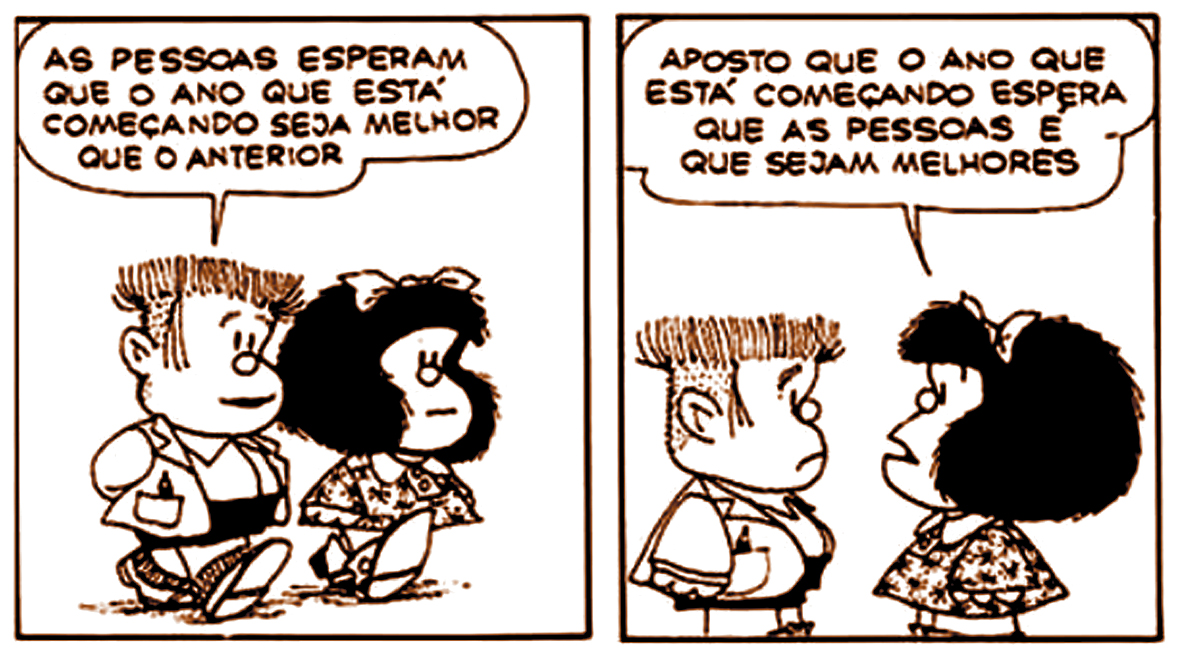
\includegraphics[width=0.75\textwidth]{figuras/mafalda}
%    \begin{flushleft}
%    \flushleft{Fonte: 
%    Elaborado pelo autor.}
%    \end{flushleft}
%    \label{fig:mafalda}
%}
%\end{figure}


%Exemplo de uso de tabela no Latex (Tabela~\ref{tab:tabelaModelo}). Ver página %72 do Manual de Normalização de Trabalhos Acadêmicos do IFCE.
%\begin{table}[th]
%    \centering
%    \caption{Legenda da Tabela no Topo.}
%    \label{tab:tabelaModelo}
%    \begin{tabular}{llll}
%    & Nota mínima & Nota máxima & Nota média\\\hline
%    Ciências Humanas (CH)     & 324,8       & 862,1       & 546,5\\
%    Ciências da Natureza (CN) & 330,6       & 876,4       & 482,2\\
%    Linguagens e Códigos (LC) & 306,2       & 814,2       & 507,9\\
%    Matemática (MT)           & 318,5       & 973,6       & 473,5\\ \hline  
%    \end{tabular}
%    \begin{flushleft}
%    \flushleft{Fonte: 
%    Instituto Brasileiro de Geografia e Estatística - IBGE.}
%    \end{flushleft}
%\end{table}

\chapter{TRABALHOS RELACIONADOS}
\label{Trabalhos Relacionados}

O \textit{MongoDB} é 

\begin{itemize}
    \item MySQL and NoSQL database comparison for IoT application (rautmare2016)
    
        \begin{itemize}
            \item Comparação de performance entre o  MongoDB e o MySql
            \item Comparação de tempo de execução por quantidade de dados em operações leitura e escrita
            \item Comparação de tempo de execução por threads em operações de leitura e escrita
        \end{itemize}
        
    \item Performance Benchmarking and Comparison of Cloud-Based Databases MongoDB (NoSQL) Vs MySQL (Relational) using YCSB (pandey2020performance)
    
        \begin{itemize}
            \item Comparação de performance entre o  MongoDB e o MySql
            \item Comparação de tempo de execução por threads em operações de leitura e escrita
            \item Comparação de throughput (operações/segundo) em operações de leitura e escrita
            \item Comparação de latência média por quantidade de operações em operações de leitura e escrita
            \item Comparação de latência por throughput em operações de leitura e escrita
            \item Comparação de throughput por threads
        \end{itemize}
        
    \item Performance Comparison of CRUD Operations in IoT based Big Data Computing (seo2017performance)
    
        \begin{itemize}
            \item Comparação de performance entre o  MongoDB e o MySql
            \item Comparação de tempo de execução por quantidade de dados em operações leitura e escrita
        \end{itemize}
        
    \item MVM: MySQL Versus MongoDB (grover2016mvm)
    
        \begin{itemize}
            \item Comparação de performance entre o  MongoDB e o MySql
            \item Comparação de tempo de execução por quantidade de dados em operações leitura e escrita
        \end{itemize}
        
    \item A PERFORMANCE COMPARISON BETWEEN ORACLE AND MONGODB (moreno2016performance)
    
        \begin{itemize}
            \item Comparação de performance entre o MongoDB e Oracle
            \item Comparação de tempo de execução por quantidade de dados em operações leitura e escrita
        \end{itemize}
        
    \item Comparison of SQL, NoSQL and NewSQL Databases for Internet of Things (fatima2016)
    
        \begin{itemize}
            \item Comparação de performance entre o  MongoDB, o MySql e VoltDB (NewSQL)
            \item Comparação de tempo de execução por quantidade de dados em operações leitura e escrita
            \item Comparação por cliente único e múltiplo para operações únicas ou múltiplas
            \item Utiliza dados de sensores (MG to GB) para simular ambiente de internet das coisas
        \end{itemize}
        
    \item MongoDB, CouchBase: Performance Comparison for Image Dataset (chopade2017)
    
        \begin{itemize}
            \item Comparação de performance entre dois banco de dados NoSQL: MongoDB e CouchBase
            \item Comparação de tempo de execução por quantidade de dados em operações leitura e escrita
            \item Utiliza imagens como dados de teste
        \end{itemize}
        
    \item Performance Comparison of Two Database Management Systems: MySQL vs MongoDB (ansari2018performance)
    
        \begin{itemize}
            \item Comparação de performance entre o  MongoDB e o MySql
            \item Comparação de tamanho dos dados armazenados por quantidade de registros
            \item Comparação de tempo de execução por quantidade de registros em simples e múltiplas operações de CRUD
        \end{itemize}
        
    \item MongoDB and Oracle NoSQL: A technical critique for design decisions (anand2016mongodb)
    
        \begin{itemize}
            \item Descreve as diferenças entre dois bancos de dados NoSQL: o  MongoDB e o Oracle NoSQL
        \end{itemize}
\end{itemize}
\chapter{\textit{METODOLOGIA}}
\label{Metodologia}

Este trabalho apresenta uma pesquisa de abordagem qualitativa, de natureza aplicada, visando amenizar os problemas de busca, junção e remoção em documentos normalizados, no banco de dados \textit{MongoDB}. Para isso, foi desenvolvido um \textit{framework} denominado de \textit{Alpha Restful}, que foi projetado para a linguagem \textit{JavaScript}, para o ambiente de execução \textit{Node JS}.

% O foco do \textit{MongoDB} é o armazenamento de dados desnormalizados, disponibilizando diversas funcionalidades para a sua manipulação. Por essa razão, operações de busca e junção de documentos normalizados precisam, as vezes, serem implementadas de forma menos intuitiva e mais trabalhosa, em comparação com o SQL. Visando amenizar os problemas apresentados, foi desenvolvido um \textit{framework} denominado de \textit{Alpha Restful}. Tal ferramenta foi projetada para a linguagem \textit{JavaScript}, no ambiente de execução \textit{Node JS}, utilizando internamente o \textit{MongoDB} e o \textit{Mongoose}.

O \textit{Alpha Restful} facilita e automatiza diversas funcionalidades para o desenvolvimento de aplicações com \textit{MongoDB}. Por esta razão, dentre as funcionalidades disponíveis nesse \textit{framework}, apenas cinco\footnote{As 5 funcionalidades são: Junção de Documentos; Buscas filtradas em Documentos Relacionados; Remoção em Cascata de Documentos Relacionados; Relação de Dependência Entre os Documentos; Remoção de Identificadores Apontando para Lixo} foram selecionadas e analisadas neste trabalho, pois tais funções melhoram o processo de desenvolvimento de aplicações, através da manipulação de dados normalizados.

O estudo avalia, principalmente, a facilidade de desenvolver as cinco funcionalidades selecionadas, com o uso de algumas ferramentas de mercado, em comparação com o \textit{framework} apresentado. Também é avaliado a facilidade, utilidade e os recursos disponíveis nas ferramentas de mercado em comparação com o \textit{Alpha Restful}. Além da avaliação qualitativa, foi obtido um resultado quantitativo (para a funcionalidade Buscas Filtradas em Documentos Relacionados), onde pode ser observado uma redução na quantidade de linhas de código, com a utilização da solução proposta.

Foram utilizados procedimentos experimentais para a análise de cada funcionalidade. Para tal, codificações em \textit{JavaScript} foram desenvolvidas, a fim de extrair o quão fácil e intuitivo as implementações são. Além disso, pôde-se observar as particularidades de cada código, em relação aos conhecimentos técnicos necessários, sobre os comandos disponíveis na ferramenta.

Após a apresentação dos resultados alcançados pelos procedimentos realizados, a pesquisa objetiva caracterizar o \textit{Alpha Restful}, observando como ele apresenta melhorias para as situações apresentadas pelas outras ferramentas comparadas. Além disso, objetiva-se demonstrar os recursos disponíveis no \textit{Alpha Restful}, destacando suas vantagens e utilidade.

O \textit{Alpha Restful} disponibiliza tais funcionalidades através de um conceito apelidado de ``sincronizaçao'', representado por um objeto denominado de ``\textit{sync}''. A sincronização é o estabelecimento de uma conexão lógica entre um atributo de uma entidade com outra entidade. Uma das formas de se estabelecer essa conexão é através do armazenamento de identificadores de outros documentos. Isso é equivalente ao uso de \textit{foreign key} no modelo relacional. Uma sincronização pode ocorrer, tanto na modelagem das entidades, quanto de forma dinâmica, durante ou depois de uma pesquisa.

Uma vez que duas entidades estão sincronizadas, diversas opções podem ser definidas no objeto ``\textit{sync}''. Cada uma delas aciona eventos que esperam uma das duas entidades serem chamadas por algum método presente no \textit{framework}. Tanto atributos reais (presentes no banco de dados) quanto atributos dinâmicos (não presentes no banco de dados, pois é criado dinamicamente em memória) podem ser alvo de uma sincronização. Um exemplo de atributo dinâmico será demonstrado na seção \ref{subsubsection: relacionamento-inverso}, quando for explicado o funcionamento do relacionamento inverso. Esses atributos dinâmicos são tratados como se eles existissem dentro do banco de dados, sendo possível utilizá-los em pesquisas. Esse tipo de atributo pode ser definido, tanto na modelagem da entidade, quanto dinamicamente na chamada de uma pesquisa ou junção de documentos.

Na seção seguinte, os detalhes da metodologia, bem como os resultados, exemplos e comparação serão apresentados.

%%%%% REMOVIDO %%%%%
% A fim de demonstrar e justificar a importância da ferramenta desenvolvida, bem como demonstrar de que forma os problemas apresentados foram solucionados ou amenizados, o capítulo \ref{Resultados} apresenta um comparativo de como cada uma das 5 funcionalidades escolhidas podem ser implementadas com outras ferramentas já disponíveis no mercado, além de demonstrar quais os problemas ou dificuldades são enfrentadas usando tais ferramentas e como a utilização do \textit{Alpha Restful} pode resolver ou amenizar essas problemáticas. A fim de facilitar a apresentação do comparativo, na próxima seção será mostrado um conjunto de documentos exemplo que serão usados como base para explicar como cada funcionalidade pode manipular esses dados.
%%%%% REMOVIDO %%%%%

%diminuir as frases

%%%%% REMOVIDO %%%%%
% Para as duas primeiras funcionalidades, é apresentado, com a demonstração de exemplos práticos do código fonte, como outras ferramentas, presentes no \textit{MongoDB} ou no \textit{Mongoose}, podem ser utilizadas, bem como as vantagens e desvantagens de cada abordagem, demonstrando quais problemas são persistidos em cada uma delas. Após essa demonstração, será apresentado (também com a utilização de exemplos práticos de código fonte) como essa mesma função pode ser feita utilizando o \textit{Alpha Restful}, mostrando como o \textit{framework} resolve ou ameniza os problemas apresentados anteriormente, bem como quais opções a mais estão disponíveis por meio desta ferramenta. Para as demais funcionalidades, é apresentado uma breve descrição de como elas podem manualmente ser implementadas usando o \textit{MongoDB} e logo após é apresentado como é possível, através do \textit{Alpha Restful}, resolver tal necessidade de maneira mais automatizada.
%%%%% REMOVIDO %%%%%

% \footnote{Emanuel: lembrar que o trabalho já está pronto, então ao invés de usar termos como irá apresentar, irá mostrar, vc usa termos como apresenta, mostra, expõe}
\chapter{RESULTADOS}
\label{Resultados}

O \textit{Alpha Restful} facilita e automatiza a implementação de 5 funcionalidades que, por causa dos motivos descritos anteriormente, podem ser complexas de serem desenvolvidas no \textit{MongoDB} sem o uso de um framework. Para cada funcionalidade, será exemplicado sua implementação sem o uso do \textit{Alpha Restful} e, posteriormente, com o uso desse framework. Para o detalhamento dessas funcionalidades, será utilizado como base a modelagem de dados exemplificada pelos seguintes documentos normalizados:

\begin{lstlisting}[language=json, caption={Documento da Casa de Número 1B}]
{
    "_id": 10,
    "rua": "Rua Castelo branco",
    "numero": "1B"
}
\end{lstlisting}

\begin{lstlisting}[language=json, caption={Documento da Casa de Número 1089}]
{
    "_id": 20,
    "rua": "Rua Pompel",
    "numero": "1089"
}
\end{lstlisting}

\newpage

\begin{lstlisting}[language=json, caption={Documento da Pessoa \textit{Eduardo}}]
{
    "_id": 2,
    "nome": "Eduardo",
    "idade": 40,
    "casas": [{
        "_id": ObjectId("5e66cb581766a2056c48145f"),
        "id": 20,
        "valorMensal": 300,
        "quantidadeMeses": 8
    }]
}
\end{lstlisting}

\begin{lstlisting}[language=json, caption={Documento da Pessoa \textit{Emanuel}}]
{
    "_id": 1,
    "nome": "Emanuel",
    "idade": 21,
    "casas": [
        {
            "_id": ObjectId("5e66cb3a7216361ff05b3b8f"),
            "id": 10,
            "valorMensal": 200,
            "quantidadeMeses": 12
        },
        {
            "_id": ObjectId("5e66cb43534f8a1944cdb028"),
            "id ": 20,
            "valorMensal": 400,
            "quantidadeMeses": 24
        }
    ]
}
\end{lstlisting}

\section{Junção de Documentos}

Assim como foi visto na seção \textit{2.2.6}, as vezes, documentos que foram completamente ou parcialmente normalizados precisam ser unidos por meio de seus relacionamentos. A junção de documentos pode ser feita de maneira automática com a utilização do \textit{\$lookup}, \textit{DBRef}, ou do \textit{populate} do \textit{Mongoose}, porém estas abordagens possuem algumas limitações.

\subsection{\textit{\$lookup}}

O \textit{\$lookup} é uma operação disponibilizada de forma oficial pelo \textit{MongoDB}. Tal operação se responsabiliza por unir dois ou mais documentos relacionados. Após tal união, pesquisas podem ser realizadas sobre esses dados e valores podem ser agrupados e ordenados. Para unirmos as coleções de Pessoas e Casas, ignorando os atributos de relacionamento, a seguite operação poderia ser feita:

\begin{lstlisting}[style=ES6, caption={Junção de Documentos com \textit{\$lookup} Com Omissão}]
    let UNIAO = await db.collection("pessoas").aggregate([
        { $lookup: {
            from: "casas",
            localField: "casas.id",
            foreignField: "_id",
            as: "casas"
        }}
    ]).toArray()
\end{lstlisting}

A opção ``\textit{from}'' contém o nome da coleção de documentos relacionada com a coleção de pessoas. O ``\textit{localField}'' contém o nome do atributo que possui o identificador da entidade relacionada, contido no documento da coleção de pessoas. O ``\textit{foreignField}'' contém o nome do atributo que possui o identificador da entidade relacionada, contido no documento da coleção de casas. A opção ``\textit{as}'' possui o nome do atributo que conterá todos os atributos da entidade relacionada. Opós essa operação, a  variável ``UNIAO'' conterá o seguinte resultado:

\newpage

\begin{lstlisting}[language=json, caption={Junção de Documentos com Omissão}]
[{
    "_id": 1,
    "nome": "Emanuel",
    "idade": 21,
    "casas": [
        {
            "_id": 10,
            "rua": "Rua Castelo Branco",
            "numero": "1B"
        },
        {
            "_id": 20,
            "rua": "Rua Pompel",
            "numero": 1089
        }
    ]
},
{
    "_id": 2,
    "nome": "Eduardo",
    "idade": 40,
    "casas": [{
        "_id": 20,
        "rua": "Rua Pompel",
        "numero": "1089"
    }]
}]
\end{lstlisting}

Observa-se que os atributos ``valorMensal'' e ``quantidadeMeses'' não encontram-se no resultado da operação feita anteriormente. Isso ocorre porque o \textit{\$lookup} sobrescreve o atributo ``casas'' por todos os atributos presentes no documento de Casa. Pode-se observar também que o identificador (\textit{\_id}) da relação é substituída pelo identificador presente na própria entidade. Essa omisão de atributos pode ser um incoveniente, caso seja necessário obter ou realizar operações nos atributos que estão sendo omitidos.

Para a utilização do \textit{\$lookup} sem a omissão de tais valores, uma codificação mais complexa e menos intuitiva tornaria-se necessária. Uma possível codificação para isto seria:

\begin{lstlisting}[style=ES6, caption={Junção de Documentos sem Omissão}]
    let UNIAO = await db.collection("pessoas").aggregate([
        { $unwind: "$casas" },
        { $lookup: {
            from: "casas",
            let: { casas: "$casas" },
            pipeline: [
                { $match: { $expr: {
                    $eq: [ "$_id", "$$casas.id" ]
                }}},
                { $addFields: {
                    _id: "$$casas._id",
                    id: "$$casas.id",
                    valorMensal: "$$casas.valorMensal",
                    quantidadeMeses: "$$casas.quantidadeMeses"
                }}
            ],
            as: "casas"
        }},
        { $group: {
            _id: {
                _id: "$_id",
                nome: "$nome",
                idade: "$idade"
            },
            casas: { $push: "$casas" }
        }},
        { $project: {
            _id: "$_id._id",
            nome: "$_id.nome",
            idade: "$_id.idade",
            casas: { $reduce: {
                input: "$casas",
                initialValue: [],
                in: { $concatArrays: [ "$$value", "$$this" ] }
            }}
        }}
    ]).toArray()
\end{lstlisting}

Para adicionar os atributos de relacionamento dentro dos objetos de casa, tornou-se necessário utilizar-se de alguns artifícios do \textit{MongoDB}, manipulando a união em baixo nível. Isso tornou-se necessário pois os identificadores das casas estão dentro de uma lista. Se uma pessoa podesse, no máximo, ter uma única casa, uma codificação mais simples poderia ser realizada. Bastaria para isso usar o primeiro exemplo de código apresentado sobre \textit{\$lookup} e apenas colocar na opção \textit{``as''} do \textit{\$lookup} um outro caminho que não sobrescreveria nenhum atributo já existente. Após a execução do código anterior, a variável ``UNIAO'' obterá o seguinte resultado:

\newpage

\begin{lstlisting}[language=json, caption={Junção de Documentos com \textit{\$lookup}}]
[{
    "_id": 1,
    "nome": "Emanuel",
    "idade": 21,
    "casas": [
        {
            "_id": ObjectId("5e66cb3a7216361ff05b3b8f"),
            "id": 10,
            "rua": "Rua Castelo Branco",
            "numero": "1B",
            "valorMensal": 200,
            "quantidadeMeses": 12
        },
        {
            "_id": ObjectId("5e66cb43534f8a1944cdb028"),
            "id": 20,
            "rua": "Rua Pompel",
            "numero": 1089,
            "valorMensal": 400,
            "quantidadeMeses": 24
        }
    ]
},
{
    "_id": 2,
    "nome": "Eduardo",
    "idade": 40,
    "casas": {
        "_id": ObjectId("5e66cb581766a2056c48145f"),
        "id": 20,
        "rua": "Rua Pompel",
        "numero": "1089",
        "valorMensal": 300,
        "quantidadeMeses": 8
    }
}]
\end{lstlisting}

Pode-se observar que a implementação feita para obter uma simples junção de documentos pode ser complexa, sendo que tais operações são mais simples e intuitivas usando o SQL. A complexidade aumenta caso deseje-se fazer uniões em cascata, ou seja, unir documentos, que foram unidos com outros documentos. Quanto maior for o nível de uniões a serem feitas, mais complexo o código fica, podendo facilitar a ocorrência de erros humanos de codificação.

\subsection{\textit{DBRef}}

O \textit{DBRef} é um padrão para referenciar outros documentos de outras coleções. Essa convenção tem a finalidade de armazenar o nome da coleção relacionada (\textit{\$ref}), o identificador do documento (\textit{\$id}) e o nome do banco de dados na qual essa coleção está contida (\textit{\$db}). Se o \textit{\$db} não for informado, assume-se que a coleção está presente no banco de dados do documento que o \textit{DBRef} reside. No exemplo a qual está sendo tratado, as pessoas registradas no sistema poderiam se relacionar com suas casas da seguinte forma:

\begin{lstlisting}[language=json, caption={Documento da Pessoa \textit{Eduardo}}]
{
    "_id": 2,
    "nome": "Eduardo",
    "idade": 40,
    "casas": [{
        "_id": ObjectId("5e66cb581766a2056c48145f"),
        "$id": 20,
        "$ref": "casas",
        "valorMensal": 300,
        "quantidadeMeses": 8
    }]
}
\end{lstlisting}

\newpage

\begin{lstlisting}[language=json, caption={Documento da Pessoa \textit{Emanuel}}]
{
    "_id": 1,
    "nome": "Emanuel",
    "idade": 21,
    "casas": [
        {
            "_id": ObjectId("5e66cb3a7216361ff05b3b8f"),
            "$id": 10,
            "$ref": "casas",
            "valorMensal": 200,
            "quantidadeMeses": 12
        },
        {
            "_id": ObjectId("5e66cb43534f8a1944cdb028"),
            "$id": 20,
            "$ref": "casas",
            "valorMensal": 400,
            "quantidadeMeses": 24
        }
    ]
}
\end{lstlisting}

Pode-se obervar que o \textit{DBRef} é utilizado quando o identificador do documento relacionado é armazenado em \textit{\$id} e quando está presente o atributo \textit{\$ref}, contendo o nome da coleção. Essa padronização é utilizada por algumas bibliotecas e frameworks para disponibilizar recursos de união de documentos automáticas. Nesse caso, uniões de uniões de documentos poderiam ser feitas automaticamente de forma simples, dependendo da ferramenta que está sendo utilizada para o desenvolvimento. Esses recursos provenientes do \textit{DBRef} não está disponível em todas as linguagens, e cada biblioteca ou framework pode tratar isso de forma diferente.

Os atributos de relacionamento (``\_id'', ``valorMensal'', ``quantidadeMeses'') não necessariamente são tratados pela biblioteca ou framework utilizado, podendo eles serem ignorados. Nesse caso, os dados precisariam ser remodelados para extrair esses atributos para outro lugar. Uma maneira de fazer isso seria criar uma nova coleção de documentos auxiliares. Tais documentos armazenariam os atributos de relacionamento e o identificador da entidade relacionada. Depois seria necessário fazer um \textit{DBRef} com o novo documento criado. Caso esses documentos auxiliares sejam aplicados na modelagem exemplo trabalhada nessa seção, os documentos se pareceriam com:

\begin{lstlisting}[language=json, caption={Documento da Pessoa \textit{Eduardo}}]
{
    "_id": 2,
    "nome": "Eduardo",
    "idade": 40,
    "casas": [{
        "$id": ObjectId("5e66cb581766a2056c48145f"),
        "$ref": "relacionamento_pessoas_casas"
    }]
}
\end{lstlisting}

\begin{lstlisting}[language=json, caption={Documento da Pessoa \textit{Emanuel}}]
{
    "_id": 1,
    "nome": "Emanuel",
    "idade": 21,
    "casas": [
        {
            "$id": ObjectId("5e66cb3a7216361ff05b3b8f"),
            "$ref": "relacionamento_pessoas_casas"
        },
        {
            "$id": ObjectId("5e66cb43534f8a1944cdb028"),
            "$ref": "relacionamento_pessoas_casas"
        }
    ]
}
\end{lstlisting}

\newpage

\begin{lstlisting}[language=json, caption={Documento do Relacionamento da Pessoa \textit{Eduardo} Com Sua Casa}]
{
    "_id": ObjectId("5e66cb581766a2056c48145f"),
    "valorMensal": 300,
    "quantidadeMeses": 8,
    "casa": {
        "$id": 20,
        "$ref": "casas"
    }
}
\end{lstlisting}

\begin{lstlisting}[language=json, caption={Documento do Relacionamento da Pessoa \textit{Emanuel} Com Sua Primeira Casa}]
{
    "_id": ObjectId("5e66cb3a7216361ff05b3b8f"),
    "valorMensal": 200,
    "quantidadeMeses": 12,
    "casa": {
        "$id": 10,
        "$ref": "casas"
    }
}
\end{lstlisting}

\begin{lstlisting}[language=json, caption={Documento do Relacionamento da Pessoa \textit{Emanuel} Com Sua Segunda Casa}]
{
    "_id": ObjectId("5e66cb43534f8a1944cdb028"),
    "valorMensal": 400,
    "quantidadeMeses": 24,
    "casa": {
        "$id": 20,
        "$ref": "casas"
    }
}
\end{lstlisting}

\newpage

\begin{lstlisting}[language=json, caption={Documento da Casa de Número 1B}]
{
    "_id": 10,
    "rua": "Rua Castelo branco",
    "numero": "1B"
}
\end{lstlisting}

\begin{lstlisting}[language=json, caption={Documento da Casa de Número 1089}]
{
    "_id": 20,
    "rua": "Rua Pompel",
    "numero": "1089"
}
\end{lstlisting}

Esses documentos auxiliares para representar o relacionamento de pessoa com casa são necessários caso o \textit{DBRef} esteja sendo utilizado e as ferramentas de desenvolvimento usadas estejam ignorando os atributos de relacionamento. Dependendo das bibliotecas e frameworks utilizados, pode ser que esses documentos auxiliares não sejam necessários, e os dados desses documentos possam ser inseridos no documento principal. A abordagem a ser utilizada dependerá da linguagem e da plataforma que está sendo utilizada. Se o ambiente de execução utilizado suportar tal estratégia, seria possível relacionar as pessoas com suas casas por meio de uma modelagem parecida com isso:

\begin{lstlisting}[language=json, caption={Documento da Pessoa \textit{Eduardo}}]
{
    "_id": 2,
    "nome": "Eduardo",
    "idade": 40,
    "casas": [{
        "_id": ObjectId("5e66cb581766a2056c48145f"),
        "valorMensal": 300,
        "quantidadeMeses": 8,
        "casa": {
            "$id": 20,
            "$ref": "casas"
        }
    }]
}
\end{lstlisting}

\begin{lstlisting}[language=json, caption={Documento da Pessoa \textit{Emanuel}}]
{
    "_id": 1,
    "nome": "Emanuel",
    "idade": 21,
    "casas": [
        {
            "_id": ObjectId("5e66cb3a7216361ff05b3b8f"),
            "valorMensal": 200,
            "quantidadeMeses": 12,
            "casa": {
                "$id": 10,
                "$ref": "casas"
            }
        },
        {
            "_id": ObjectId("5e66cb43534f8a1944cdb028"),
            "valorMensal": 400,
            "quantidadeMeses": 24,
            "casa": {
                "$id": 20,
                "$ref": "casas"
            }
        }
    ]
}
\end{lstlisting}

\begin{lstlisting}[language=json, caption={Documento da Casa de Número 1B}]
{
    "_id": 10,
    "rua": "Rua Castelo branco",
    "numero": "1B"
}
\end{lstlisting}

\newpage

\begin{lstlisting}[language=json, caption={Documento da Casa de Número 1089}]
{
    "_id": 20,
    "rua": "Rua Pompel",
    "numero": "1089"
}
\end{lstlisting}

Essa última abordagem apresentada possui a vantagem de não existir um documento auxiliar intermediando o relacionamento. Isso é útil por diminuir o armazenamento e por permitir que consultas mais complexas sejam mais simples de se implementar.

Assim como explicado anteriormente, o \textit{DBRef} pode permitir que operações de união de documentos ocorram de forma mais simples e automática, caso o ambiente de execução utilizado disponibilize tais opções para os BSONs que seguem seu padrão. Apesar dos benefícios, operações mais complexas como, por exemplo, buscas sobre valores presentes em vários documentos, podem não estar disponíveis via \textit{DBRef}. Além disso, operações como o \textit{\$lookup} podem exigir que o \textit{DBRef} seja convertido para um outro formato antes de tais operações serem realizadas. 

Por causa disso, o uso do \textit{DBRef} pode exigir codificações mais complexas em determinadas situações onde a biblioteca ou framework não daria suporte. Por essas razões que, dependendo das ferramentas disponibilizadas pelo ambiente de execução, bem como das necessidades do projeto, pode ser que o uso de uma referencia manual de outros documentos seja uma melhor escolha do que o \textit{DBRef}.

\subsection{\textit{Populate} do \textit{Mongoose}}

O \textit{Mongoose} é uma biblioteca feita para \textit{Node JS}, que disponibiliza algumas funcionalidades a mais para o \textit{MongoDB}, principalmente relacionadas à modelagem dos dados. Através dessa ferramenta, torna-se possível criar \textit{schemas} para os dados a serem armazenados. Esses \textit{schemas} permitem que a estrutura do BSON de cada documento seja padronizada e obeceça as regras de estrutura definidos pelo programador. Para o exemplo que está sendo apresentado, os seguintes \textit{schemas} podem ser utilizados:

\newpage

\begin{lstlisting}[style=ES6, caption={Definição de \textit{Schemas} no \textit{Mongoose}}]
    const PessoaSchema = new mongoose.Schema({
        _id: Number,
        nome: String,
        idade: Number,
        casas: [{
            _id: mongoose.Schema.Types.ObjectId,
            id: {
                type: Number,
                ref: "casas"
            },
            valorMensal: Number,
            quantidadeMeses: Number
        }]
    })
    const Pessoa = db.model("pessoas", PessoaSchema)

    const CasaSchema = new mongoose.Schema({
        _id: Number,
        rua: String,
        numero: String
    })
    const Casa = db.model("casas", CasaSchema)
\end{lstlisting}

Um dos recursos disponibilizados pelo \textit{Mongoose} é o \textit{populate}. Este recurso substitui o \textit{DBRef} e o \textit{\$lookup} para operações de busca, seguido de união de documentos. A restrição do \textit{populate} em comparação com o \textit{\$lookup} é que no \textit{\$lookup} é possível realizar buscas sobre os dados dos documentos unidos, enquanto que no \textit{populate} a busca deve ocorrer apenas sobre os dados originais do documento. Se desconsiderarmos essa ``limitação'', o \textit{populate} é mais simples de se usar do que o \textit{\$lookup}, além de disponibilizar novas opções e recursos. Atualmente, o \textit{Mongoose} está disponível apenas para o \textit{Node JS}, que é exatamanete o escopo a qual esse trabalho se propõe em atual. Para que os documentos da coleção de Pessoa e Casa sejam unidos com o \textit{populate}, seria necessário fazer uma codificação parecida com isso:

\begin{lstlisting}[style=ES6, caption={União de Documentos Com o \textit{Populate}}]
  let UNIAO = await Pessoa.find({}).populate("casas.id").exec()
\end{lstlisting}

Com apenas uma única linha, os dois documentos foram unidos, mantendo os atributos de relacionamento. Após a execução do código anterior, a variável ``UNIAO'' terá o seguinte resultado:

\begin{lstlisting}[language=json, caption={Junção de Documentos Com o \textit{Populate}}]
[{
    "_id": 1,
    "nome": "Emanuel",
    "idade": 21,
    "casas": [
        {
            "_id": ObjectId("5e66cb3a7216361ff05b3b8f"),
            "id": {
                "_id": 10,
                "rua": "Rua Castelo Branco",
                "numero": "1B"
            },
            "valorMensal": 200,
            "quantidadeMeses": 12
        },
        {
            "_id": ObjectId("5e66cb43534f8a1944cdb028"),
            "id": {
                "_id": 10,
                "rua": "Rua Pompel",
                "numero": 1089
            },
            "valorMensal": 400,
            "quantidadeMeses": 24
        }
    ]
},
{
    "_id": 2,
    "nome": "Eduardo",
    "idade": 40,
    "casas": {
        "_id": ObjectId("5e66cb581766a2056c48145f"),
        "id": {
            "_id": 10,
            "rua": "Rua Pompel",
            "numero": 1089
        },
        "valorMensal": 300,
        "quantidadeMeses": 8
    }
}]
\end{lstlisting}

Pode-se observar que os valores de casa foram preenchidos no atributo onde encontra-se o identificador do documento. Por causa dessa característica do \textit{populate}, pode ser mais intuitivo, para este caso, remodelar a entidade de pessoa, para que o atributo ``\textit{id}'' seja renomeado para, por exemplo, ``casa''. Nesse caso, os resultados sairiam com o seguinte formato:

\begin{lstlisting}[language=json, caption={Junção de Documentos Com o \textit{Populate}}]
[{
    "_id": 1,
    "nome": "Emanuel",
    "idade": 21,
    "casas": [
        {
            "_id": ObjectId("5e66cb3a7216361ff05b3b8f"),
            "casa": {
                "_id": 10,
                "rua": "Rua Castelo Branco",
                "numero": "1B"
            },
            "valorMensal": 200,
            "quantidadeMeses": 12
        },
        {
            "_id": ObjectId("5e66cb43534f8a1944cdb028"),
            "casa": {
                "_id": 10,
                "rua": "Rua Pompel",
                "numero": 1089
            },
            "valorMensal": 400,
            "quantidadeMeses": 24
        }
    ]
},
{
    "_id": 2,
    "nome": "Eduardo",
    "idade": 40,
    "casas": {
        "_id": ObjectId("5e66cb581766a2056c48145f"),
        "casa": {
            "_id": 10,
            "rua": "Rua Pompel",
            "numero": 1089
        },
        "valorMensal": 300,
        "quantidadeMeses": 8
    }
}]
\end{lstlisting}

\subsection{União de Documentos de Forma Manual}

Caso haja a necessidade de obter um maior controle na união dos documentos, ou se os recursos de união automático não forem satisfatório o suficiente para as necessidades da aplicação, é possível realizar uma união de forma manual. Um exemplo de uma codificação manual de junção de documentos encontra-se a seguir:

\newpage

\begin{lstlisting}[style=ES6, caption={Junção Manual dos Documentos de Pessoa com Casa}]
    let pessoas = await db.collection("pessoas")
        .find({}).toArray();
    
    for (let p of pessoas) {
        for (let i = 0; i < p.casas.length; i++) {
            let c = p.casas[i];
    
            let casa = (await db.collection("casas").find({
                "_id": c.id
            }).toArray())[0];
    
            p.casas[i] = {
                ...casa,
                ...c
            };
        }
    }
\end{lstlisting}

Ao final desse código, a variável ``pessoas'' terá a junção dos documentos da coleção de Pessoa e Casa. Tal variável teria o seguinte resultado:

\newpage

\begin{lstlisting}[language=json, caption={Junção de Documentos de Forma Manual}]
[{
    "_id": 1,
    "nome": "Emanuel",
    "idade": 21,
    "casas": [
        {
            "_id": ObjectId("5e66cb3a7216361ff05b3b8f"),
            "id": 10,
            "rua": "Rua Castelo Branco",
            "numero": "1B",
            "valorMensal": 200,
            "quantidadeMeses": 12
        },
        {
            "_id": ObjectId("5e66cb43534f8a1944cdb028"),
            "id": 20,
            "rua": "Rua Pompel",
            "numero": 1089,
            "valorMensal": 400,
            "quantidadeMeses": 24
        }
    ]
},
{
    "_id": 2,
    "nome": "Eduardo",
    "idade": 40,
    "casas": {
        "_id": ObjectId("5e66cb581766a2056c48145f"),
        "id": 20,
        "rua": "Rua Pompel",
        "numero": "1089",
        "valorMensal": 300,
        "quantidadeMeses": 8
    }
}]
\end{lstlisting}

%Observa-se que em um ambiente real, vários documentos %precisariam ser unidos, deixando o código cada vez mais complexo.

\subsection{Usando o \textit{Alpha Restful} Para Unir Documentos}

O \textit{Alpha Restful} possui sua própria implementação para unir os documentos. Internamente, os documentos sempre são unidos de forma manual. A vantagem de se utilizar o \textit{Alpha Restful} é que ele disponibiliza duas novas funcionalidades que não estão diretamente disponíveis pelos métodos descritos anteriormente:

\begin{itemize}
	\item Relacionamento inverso
	\item Relacionamento inverso de um relacionamento inverso
\end{itemize}

Para que as funcionalidades do \textit{framework} sejam disponibilizadas, o \textit{Alpha Restful} utiliza os \textit{schemas} do \textit{Mongoose}, em conjunto com especificações de sincronização (\textit{sync}) entre as entidades. Essas especificações de sincronização permitem que entidades sejam relacionadas entres si baseado em identificadores e em outros tipos de relacionamentos (que não serão explicados por fugir do escopo desse trabalho). No exemplo a qual está sendo trabalhado nessa seção, os \textit{schemas} e especificações de sincronização das entidades podem ser definidos no \textit{Alpha Restful} com uma codificação parecida com isso:

\newpage

\begin{lstlisting}[style=ES6, caption={Definição de \textit{Schemas} no \textit{Alpha Restful}}]
    const restful = new Restful("<nome-da-aplicacao>", {
        locale: "pt"
    })

    const Pessoa = new Entity({
        name: "Pessoa",
        resource: "pessoas",
        descriptor: {
            nome: String,
            idade: Number,
            casas: [{
                id: Number,
                valorMensal: Number,
                quantidadeMeses: Number
            }]
        },
        sync: {
            casas: {
                name: "Casa",
                fill: true
            }
        }
    })
    
    const Casa = new Entity({
        name: "Casa",
        resource: "casas",
        descriptor: {
            rua: String,
            numero: String
        }
    })
    
    restful.add(Pessoa)
    restful.add(Casa)
\end{lstlisting}

Para a união de documentos, o \textit{Alpha Restful} disponibiliza uma opção denominada de \textit{fill}. Tal opção é poderosa, pois ela pode ser utilizada sobre qualquer objeto já pesquisado ou montado, sendo possível definir, na chamada da função, relacionamentos temporários com outras entidades. Para que os documentos da coleção de Pessoa e Casa sejam unidos com o \textit{Alpha Restful}, uma codificação parecida com isso teria que ser feita:

\begin{lstlisting}[style=ES6, caption={União de Documentos Com o \textit{Alpha Restful}}]
	let pessoas = await Pessoa.model.find({}).exec()
	pessoas = await Pessoa.fill(pessoas, restful)
\end{lstlisting}

A operação de união de documentos ocorre após os objetos terem sido obtidos, por exemplo, por meio de uma busca. Nesse caso buscou-se por todas as pessoas. Após essa busca, basta chamar o método \textit{Pessoa.fill} para que os documentos sejam unidos. Como na modelagem já tinha sido definido que o atributo ``casas'' de pessoa fazia um relacionamento com a entidade ``Casa'' (através do objeto \textit{sync}), e que por padrão os documentos devem ser unidos (através da opção \textit{fill} igual a \textit{true} em \textit{sync}), apenas a chamada do método é o suficiente para realizar a união. Na versão atual do \textit{Alpha Restful} (0.7.37), o identificador da entidade relacionada precisa ser definido no atributo \textit{id}. Depois de executar o código anterior, a variável ``pessoas'' obterá o seguintes resultado:

\newpage

\begin{lstlisting}[language=json, caption={Junção de Documentos Com o \textit{Alpha Restful}}]
[{
    "_id": 1,
    "nome": "Emanuel",
    "idade": 21,
    "casas": [
        {
            "_id": ObjectId("5e66cb3a7216361ff05b3b8f"),
            "id": 10,
            "rua": "Rua Castelo Branco",
            "numero": "1B",
            "valorMensal": 200,
            "quantidadeMeses": 12
        },
        {
            "_id": ObjectId("5e66cb43534f8a1944cdb028"),
            "id": 20,
            "rua": "Rua Pompel",
            "numero": 1089,
            "valorMensal": 400,
            "quantidadeMeses": 24
        }
    ]
},
{
    "_id": 2,
    "nome": "Eduardo",
    "idade": 40,
    "casas": {
        "_id": ObjectId("5e66cb581766a2056c48145f"),
        "id": 20,
        "rua": "Rua Pompel",
        "numero": "1089",
        "valorMensal": 300,
        "quantidadeMeses": 8
    }
}]
\end{lstlisting}

\subsubsection{Relacionamento Inverso}

Uma das funcionalidades disponibilizadas pelo \textit{Alpha Restful} que, atualmente, não estão diretamente disponíveis nos outros métodos de união de documentos mostrados (com exceção do método manual), é o relacionamento inverso. Para ilustrar tal funcionalidade, pode-se analisar a situação onde seria necessário unir as duas coleções, mas unindo nos documentos de casa. Essa operação pode ser feita diretamente no método de \textit{fill}, sem a necessidade de alterar a modelagem da entidade:

\begin{lstlisting}[style=ES6, caption={União de Documentos em Relacionamento Inverso}]
    let casas = await Casa.model.find({}).exec()
    casas = await Casa.fill(casas, restful, { sync: {
        pessoas: {
            name: "Pessoa",
            syncronized: ["casas"],
            fill: true,
            jsonIgnoreProperties: "casas"
        }
    }})
\end{lstlisting}

A opção ``\textit{jsonIgnoreProperties}'', nesse caso, é responsável por ignorar o atributo ``casas'' de Pessoa. Isso é necessário para que não ocorra uma recursão infinita. Sem essa opção, as pessoas seriam preenchidas no atributo ``pessoas'', as casas seriam preenchidas no atribututo ``casas'', as pessoas seriam novamente preenchidas no atributo ``pessoas'' e assim por diante. Com a opção ``\textit{jsonIgnoreProperties}'', as casas não serão incluídas nas pessoas. Após a execução do código anterior, os documentos de Casa e Pessoa são unidos, mas tendo como base a entidade ``Casa''. Os documentos unidos estarão presentes na variável ``casas'' e teria a seguinte estrutura:

\newpage

\begin{lstlisting}[language=json, caption={Junção de Documentos em ``Casa''}]
[
    {
        "_id": 10,
        "rua": "Rua Castelo Branco",
        "numero": "1B",
        "pessoas": [
            {
                "id": 1,
                "nome": "Emanuel",
                "idade": 21
            }
        ]
    },
    {
        "_id": 20,
        "rua": "Rua Pompel",
        "numero": "1089",
        "pessoas": [
            {
                "id": 1,
                "nome": "Emanuel",
                "idade": 21
            },
            {
                "id": 2,
                "nome": "Eduardo",
                "idade": 40
            }
        ]
    }
]
\end{lstlisting}

Como na modelagem da entidade de ``Casa'' o relacionamento com pessoa não foi definido, é possível fazer essa definição na hora de realizar a união. Pode-se observar que não existe a necessidade de armazenar os identificadores das pessoas nas suas casas, o \textit{framework} consegue automaticamente identificálos, bastando apenas informar na opção ``\textit{syncronized}'' o caminho para se obter as casas por meio de uma pessoa. Caso fosse desejado obter esse comportamento por padrão, assim como ocorre em ``Pessoa'', bastaria atualizar o objeto ``\textit{sync}'' da entidade ``Casa''. Se isso for feito, a união poderia ocorrer sem a definição do relacionamento na hora da união. Nesse caso, a modelagem de Casa ficaria da seguinte forma:

\begin{lstlisting}[style=ES6, caption={Definição do \textit{Schema} de Casa}]
    const Casa = new Entity({
        name: "Casa",
        resource: "casas",
        descriptor: {
            rua: String,
            numero: String
        },
        sync: {
            pessoas: {
                name: "Pessoa",
                syncronized: ["casas"],
                fill: true,
                jsonIgnoreProperties: "casas"
            }
        }
    })
\end{lstlisting}

\subsubsection{Relacionamento Inverso do Relacionamento Inverso}

Outra funcionalidade disponibilizada pelo \textit{Alpha Restful} que, atualmente, não está disponível nos outros métodos de união de documentos mostrados (com exceção do método manual), é o relacionamento inverso do relacionamento inverso. Uma forma de ilustrar essa função é tentar obter, no documento das pessoas, a lista de moradores de uma ou mais casas que a própria pessoa também mora. Para isso, bastaria fazer um relacionamento inverso do atributo ``pessoas'' em casas:

\begin{lstlisting}[style=ES6, caption={Definição de \textit{Schemas} no \textit{Alpha Restful}}]
    const restful = new Restful("<nome-da-aplicacao>", {
        locale: "pt"
    })

    const Pessoa = new Entity({
        name: "Pessoa",
        resource: "pessoas",
        descriptor: {
            nome: String,
            idade: Number,
            casas: [{
                id: Number,
                valorMensal: Number,
                quantidadeMeses: Number
            }]
        },
        sync: {
            casas: {
                name: "Casa",
                fill: true,
                jsonIgnoreProperties: "pessoas"
            },
            residentes: {
                name: "Pessoa",
                syncronized: ["casas.pessoas"],
                fill: true,
                jsonIgnoreProperties: ["residentes", "casas"]
            }
        }
    })
    
    const Casa = new Entity({
        name: "Casa",
        resource: "casas",
        descriptor: {
            rua: String,
            numero: String
        },
        sync: {
            pessoas: {
                name: "Pessoa",
                syncronized: ["casas"],
                fill: true,
                jsonIgnoreProperties: "casas"
            }
        }
    })
    
    restful.add(Pessoa)
    restful.add(Casa)
\end{lstlisting}

Os \textit{schemas} definidos no código anterior criam em Pessoa um novo atributo (``residentes'') que contém todas as pessoas que então contidas no atributo definido em \textit{``syncronized''} que, neste caso, é o atributo ``casas.pessoas''. Pode-se observar a presença da opção ``\textit{jsonIgnoreProperties}'' no ``\textit{sync}'' das entidades. Tal opção armazena o nome do atributo (poderia ser uma lista de nomes de atributos) que será ignorado nos documentos que serão unidos. Isso é necessário para impedir uma união recursiva infinita de atributos. Da forma como a modelagem está definida, ao se unir os documentos de pessoa com casa, havera um atributo no documento de pessoa chamado de ``residentes'', que conterá todas as pessoas que moram em uma ou mais casas na qual a própria pessoa também mora. Essa união de documentos pode ser realizado por meio do seguinte código:

\begin{lstlisting}[style=ES6, caption={União de Documentos Com o \textit{Alpha Restful}}]
	let pessoas = await Pessoa.model.find({}).exec()
	pessoas = await Pessoa.fill(pessoas, restful)
\end{lstlisting}

Por causa do relacionamento inverso, que também pode se relacionar com um outro relacionamento inverso, a união de documentos por meio do \textit{Alpha Restful} é mais poderosa que as outras opções descritas anteriormente. Ao final da execução do código anterior, a variável ``pessoas'' terá o seguinte resultado:

\begin{lstlisting}[language=json, caption={Junção de Documentos Com Residentes}]
[{
    "_id": 1,
    "nome": "Emanuel",
    "idade": 21,
    "casas": [
        {
            "_id": ObjectId("5e66cb3a7216361ff05b3b8f"),
            "id": 10,
            "rua": "Rua Castelo Branco",
            "numero": "1B",
            "valorMensal": 200,
            "quantidadeMeses": 12
        },
        {
            "_id": ObjectId("5e66cb43534f8a1944cdb028"),
            "id": 20,
            "rua": "Rua Pompel",
            "numero": 1089,
            "valorMensal": 400,
            "quantidadeMeses": 24
        }
    ],
    "residentes": [
        {
            "id": 1,
            "nome": "Emanuel",
            "idade": 21,
        },
        {
            "id": 2,
            "nome": "Eduardo",
            "idade": 40,
        }
    ]
},
{
    "_id": 2,
    "nome": "Eduardo",
    "idade": 40,
    "casas": [{
        "_id": ObjectId("5e66cb581766a2056c48145f"),
        "id": 20,
        "rua": "Rua Pompel",
        "numero": "1089",
        "valorMensal": 300,
        "quantidadeMeses": 8
    }],
    "residentes": [
        {
            "id": 1,
            "nome": "Emanuel",
            "idade": 21,
        },
        {
            "id": 2,
            "nome": "Eduardo",
            "idade": 40,
        }
    ]
}]
\end{lstlisting}

\section{Buscas Filtradas em Documentos Relacionados}

O \textit{MongoDB} é nativamente capaz de realizar buscas complexas e simples dentro de um mesmo documento, mas a partir do momento que as buscas precisam ser realizadas em documentos separados que estão relacionados entre si, as pesquisas passam a ficar mais difíceis de serem realizadas. Para, por exemplo, ser feito uma busca pelas pessoas cuja a idade seja igual a 40, poderia ser realizado uma codificação parecido com isto:

\begin{lstlisting}[style=ES6, caption={Busca de Pessoas com idade igual a 40}]
    let pessoas = await db.collection("pessoas").find({
        "idade": 40
    }).toArray();
\end{lstlisting}

Ao final desse código, a variável ``pessoas'' obterá todas as pessoas na qual a idade é igual a 40. O código é simples, pois a busca ocorre dentro do próprio documento. Mas e se for desejado obter todas as casas, na qual existe pelo menos uma pessoa, que essa pessoa possui pelo menos uma casa, que nessa casa possui pelo menos uma pessoa que possui a idade igual a 40 anos?

\subsection{Usando o \textit{\$lookup}}

Para realizar a pesquisa proposta, uma abordagem possível é unir os documentos utilizando o \textit{\$lookup}, até o nível que todos os dados estariam no mesmo documento. Após essa união, seria possível fazer a pesquisa, utilizando o parâmetro ``\textit{\$match}''. A pesquisa exemplo seguinte funciona utilizando essa abordagem.

\begin{lstlisting}[style=ES6, caption={Busca em Dados Normalizados Com o \textit{\$lookup}}]
    let RESULTADO = await db.collection("casas").aggregate([
        { $lookup: {
            from: "pessoas",
            localField: "_id",
            foreignField: "casas.id",
            as: "pessoas"
        }},
        { $unwind: "$pessoas" },
        { $lookup: {
            from: "casas",
            localField: "pessoas.casas.id",
            foreignField: "_id",
            as: "pessoas.casas"
        }},
        { $unwind: "$pessoas.casas" },
        { $lookup: {
            from: "pessoas",
            localField: "pessoas.casas._id",
            foreignField: "casas.id",
            as: "pessoas.casas.pessoas"
        }},
        { $group: {
            _id: {
                _id: "$_id",
                rua: "$rua",
                numero: "$numero",
                pessoas: {
                    _id: "$pessoas._id",
                    nome: "$pessoas.nome",
                    idade: "$pessoas.idade",
                }
            },
            casas: {
                $push: "$pessoas.casas"
            }
        }},
        { $project: {
            _id: "$_id._id",
            rua: "$_id.rua",
            numero: "$_id.numero",
            pessoas: {
                _id: "$_id.pessoas._id",
                nome: "$_id.pessoas.nome",
                idade: "$_id.pessoas.idade",
                casas: "$casas"
            }
        }},
        { $group: {
            _id: {
                _id: "$_id",
                rua: "$rua",
                numero: "$numero"
            },
            pessoas: {
                $push: "$pessoas"
            }
        }},
        { $project: {
            _id: "$_id._id",
            rua: "$_id.rua",
            numero: "$_id.numero",
            pessoas: "$pessoas"
        }},
        { $match: {
            "pessoas.casas.pessoas.idade": 40
        }}
    ]).toArray()
\end{lstlisting}

Para a realização de uma pesquisa dessa complexidade, é necessário unir os documentos várias vezes, pois é necessário acessar os dados que estão dentro de uma lista (pessoas), que estão dentro de uma lista (pessoas.casas), que estão dentro de uma lista (pessoas.casas.pessoas). Por essa razão, utilizar o \textit{\$lookup} para consultas pode ser complexo.

\subsection{Pesquisa Manual}
    
Também é possível realizar a pesquisa proposta de forma manual, subdividindo a pesquisa em pesquisas menores e unindo-as em uma pesquisa que irá obter o resultado esperado. A utilização de tal abordagem para a pesquisa proposta resultaria em uma codificação parecida com isso:

\newpage

%Através de uma pesquisa pela internet, é comumente encontrado, na maioria dos fóruns pesquisados, que a pesquisa em vários documentos relacionados deve ser quebrado em várias pesquisas em cada documento. 

\begin{lstlisting}[style=ES6, caption={Busca em Dados Normalizados de Forma Manual}]
    let pessoasIdade40 = await db.collection("pessoas").find({
        "idade": 40
    }).toArray();
    
    let idsCasasPessoasIdade40 = 
    pessoasIdade40.map(p => 
        p.casas.reduce((a,c) => [...a,c.id], [])
    ).reduce((a,lid) => [...a, ...lid], []);
    
    let casasPessoasIdade40 =
    await db.collection("casas").find({
        "_id": { $in: idsCasasPessoasIdade40 }
    }).toArray();
    
    let idsCasasPessoasIdade40 = 
    casasPessoasIdade40.map(c => c._id);
    
    let pessoasCasasPessoasIdade40 = await
    db.collection("pessoas").find({
        "casas.id": { $in: idsCasasPessoasIdade40 }
    }).toArray();
    
    let idsCasasPessoasCasasPessoasIdade40 = 
    idsCasasPessoasCasasPessoasIdade40.map(p => 
        p.casas.reduce((a,c) => [...a,c.id], [])
    ).reduce((a,lid) => [...a, ...lid], []);
    
    let RESULTADO_DA_PESQUISA = await
    db.collection("casas").find({
        "_id": { $in: idsCasasPessoasCasasPessoasIdade40 }
    }).toArray();
\end{lstlisting}

Para buscar as casas, na qual existe pelo menos uma pessoa, que esta pessoa possui pelo menos uma casa, na qual esta casa possui pelo menos uma pessoa com idade igual a 40 anos, foi necessário 30 linhas com códigos.
    
O primeiro passo para realizar esta busca é de obter todas as pessoas que possui idade igual a 40 anos (linha 1 a 3). Depois, os identificadores das casas pertencentes a estas pessoas são extraídos (linhas 5 a 8). Após a extração destes identificadores, são buscados todas as casas que possui um identificador dentre esses (linhas 10 a 12). Após a busca de todas essas casas, são extraídos todos os identificares (linhas 14 a 15). Após a extração desses identificadores, são buscadas todas as pessoas que possuem alguma destas casas (linhas 17 a 20). Após a busca destas pessoas, são extraídos todos os identificadores das casas destas pessoas (linhas 22 a 25). Finalmente, as casas que possui seu identificador dentre os identificadores são buscadas, obtendo o resultado esperado pela consulta.
    
Observa-se que, tanto essa consulta, quando a consulta usando o \textit{\$lookup} e \textit{\$match}, possui apenas uma ramificação de filtros encadeados. Os códigos ficariam mais complexo com a adição de outras ramificações de filtros, utilizando-se de outras relações com outros documentos relacionados.

\subsection{Usando o \textit{Alpha Restful}}

Como visto anteriormente, realizar buscas que englobam vários documentos pode ser algo complexo. Para contornar este problema, o \textit{Alpha Restful} mapeia todos os relacionamentos normalizados dentre todos os documentos do sistema para fornecer uma sintaxe simples para se realizar pesquisas. Para ilustrar este comportamento, será considerado o exemplo de busca apresentado anteriormente. Para realizar essa pesquisa, bastaria executar o seguinte código:
    
\begin{lstlisting}[style=ES6, caption={Busca em Dados Normalizados com o \textit{Alpha Restful}}]
    let casas = await restful.query({
        "pessoas.casas.pessoas.idade": 40
    }, Casa);
\end{lstlisting}
    
Anteriormente, para a realização dessa pesquisa, foi necessário entre 30 (de forma manual) e 67 (usando \textit{\$lookup} com \textit{\$match}) linhas, mas com o \textit{Alpha Restful}, apenas 3 linhas foi o suficiente. Isso ocorre porque o \textit{Alpha Restful} consegue enxergar todos os atributos presentes em outros documentos normalizados, como se eles estivessem dentro do documento de maneira desnormalizada. A sintaxe utilizada para realizar buscas é uma extensão da sintaxe utilizada pelo \textit{Mongoose}, com a diferença de considerar nas pesquisas os atributos contidos em outros documentos relacionados.

\section{Remoção em Cascata de Documentos Relacionados}
    
No exemplo a qual está sendo abordado, pode-se supor que, por exemplo, o sistema possua uma regra de negócio que afirme que quando uma pessoa for removida, todas as casas pertencentes a essa pessoa devam ser removidas também. Para a implementação de tal regra, sem o uso de um \textit{framework}, toda vez que uma pessoa for removida, será necessário manualmente buscar por todas as casas pertencentes a esta pessoa e removê-las. O problema dessa abordagem manual é que uma coleção pode possuir vários relacionamentos com outros documentos, deixando o código cada vez mais complexo.

Pensando nisso, o \textit{Alpha Restful} disponibiliza uma opção na sincronização das entidades (\textit{sync}), que faz exatamente essa funcionalidade. Para garantir esse comportamento, é necessário apenas informar a opção \textit{deleteCascade} no atributo da entidade a qual deseja-se que seja removida automaticamente:

\begin{lstlisting}[style=ES6, caption={Modelagem de ``Casa'' com \textit{deleteCascade}}]
    const Casa = new Entity({
        name: "Casa",
        // ...
        sync: {
            pessoas: {
                name: "Pessoa",
                syncronized: ["casas"]
                fill: true,
                jsonIgnoreProperties: "casas",
                deleteCascade: true
            },
            // ...
        }
    })
\end{lstlisting}

\section{Relação de Dependência Entre os Documentos}

No exemplo a qual está sendo abordado, se uma casa não poder ser removida caso possua um relacionamento com alguma pessoa, seria necessário a verificação da existência de tal relacionamento antes de uma casa ser removida. Caso todo esse procedimento seja feito manualmente e outras entidades comecem a se relacionar com a entidade Casa, o código desta verificação ficaria cada vez mais complexo, se essa regra se repetisse para outros documentos.

Para que essa regra seja aplicada de forma mais simples, o \textit{Alpha Restful} disponibiliza no ``\textit{sync}'' uma opção que define uma relação de dependência entre os documentos. Uma relação de dependência entre documentos normalizados relacionados garante que um documento não possa ser removido se estiver presente em algum relacionamento definido como dependente. Se, por exemplo, uma casa não poder ser removida, caso possua alguma pessoa, bastaria apenas informar a opção \textit{required} no atributo da entidade a qual deseja-se criar um relacionamento de dependência (Pessoa):

\begin{lstlisting}[style=ES6, caption={Modelagem de Pessoa com \textit{required}}]
    const Pessoa = new Entity({
        name: "Pessoa",
        // ...
        sync: {
            casas: {
                name: "Casa",
                fill: true,
                jsonIgnoreProperties: "pessoas",
                required: true
            },
            // ...
        }
    })
\end{lstlisting}

\section{Identificadores Apontando para Lixo}

Um dos possíveis problemas que podem ser comuns no desenvolvimento de uma aplicação com \textit{MongoDB}, é a existência de identificadores que apontam para documentos que não existem. Isso acontece porque as entidades que possuem um identificador de outra entidade que foi removida do banco, podem continuar com esse identificador. Um exemplo que pode ser apresentado é de que se uma casa for removida, isso pode fazer com que o identificador dessa casa nos documentos da coleção de ``Pessoa'' apontará para lugar algum, pois a casa a qual tais identificadores em Pessoa apontam, já não existe mais.
    
Para que esse problema seja contornado, sem o uso de um \textit{framework}, é necessário que antes que qualquer entidade seja removida, seja realizado uma análise em todas as entidades que se relacionam com a instância a qual deseja-se remover. Após esta análise, os dados que apontariam para esta entidade que está sendo removida seriam removidos também. Com o aumento da complexidade da aplicação, esse código ficaria cada vez mais e mais complexo, pois a cada novo relacionamento entre documentos, mais alterações precisariam ser feitas no código para garantir esse comportamento. O \textit{Alpha Restful} já resolve esse problema automaticamente (bastando apenas realizar o procedimento descrito na seção 3.6). Nenhuma opção precisa ser habilitada na modelagem para que esse problema seja mitigado.

\section{\textit{deleteSync}}

Para que as funcionalidades relacionadas à remoção de entidades no \textit{Alpha Restful} possam acontecer (seções 3.3, 3.4 e 3.5), é necessário que o método \textit{restful.deleteSync} seja chamado antes que qualquer entidade ser removida. Se, por exemplo, uma casa tiver que ser removida, o seguinte código deve ser executado antes da remoção:

\begin{lstlisting}[style=ES6, caption={Antes de Remover Uma Casa}]
  await restful.deleteSync(casa._id, "Casa", Casa.syncronized)
\end{lstlisting}
\chapter{CONCLUSÃO}
\label{Conclusao}

Os bancos de dados NoSQL trazem o conceito de que o desenvolvimento de uma aplicação não precisa necessariamente estar preso às regras e limites do modelo relacional. A proposta de tais bancos inclui mudar a estrutura de como os dados são armazenados, a fim de eliminar alguma barreira imposta pelo SQL. No caso do \textit{MongoDB}, propõe-se otimizar o armazenamento e gerenciamento de dados que não precisam seguir as formas normais. Ao mesmo tempo, ele não impede a normalização, onde tal abordagem for pertinente e se demonstrar uma vantagem. Permitir que a aplicação decida sobre a normalização ou desnormalização, demonstra-se ser um bom caminho, pois possibilita que a melhor decisão possa ser tomada, dependendo das necessidades da aplicação a ser desenvolvida.

O \textit{MongoDB} disponibiliza, de forma oficial, várias recursos para auxiliar na desnormalização dos dados. Apesar disso, este trabalho demonstrou que, até mesmo em aplicações onde a desnormalização é importante, eventualmente, os dados poderão precisar estar normalizados. Quando isso acontecer, várias operações poderão ser bastante complexas de serem desenvolvidas, em comparação com o SQL. Nesse cenário, este trabalho apresentou o \textit{Alpha Restful} como uma solução capaz de minimizar tal problemática, simplificando operações complexas e disponibilizando novos recursos para elas.

%%%%% REMOVIDO %%%%%
% O \textit{Alpha Restful} é um \textit{framework} que tem uma proposta ousada. Um de seus principais objetivos de seu desenvolvimento foi fazer com que a escolha de se normalizar ou desnormalizar os dados no \textit{MongoDB}, apareça mais como uma questão de "regra de negócio", do que como uma questão estrutural profunda na forma como entidades são modeladas e buscadas. Sendo essa finalidade alcançada, a facilidade que já existe para se desnormalizar os dados no \textit{MongoDB}, também existiria para normalizá-los. Isso eliminaria um dos obstáculos que atualmente encontram-se na utilização do banco de dados: a normalização de dados do \textit{MongoDB} que, como foi demonstrado anteriormente, as vezes precisa ser feita em, pelo menos, parte dos dados armazenados, pode ser mais complexo que na desnormalização.

% Como foi demonstrado, esse objetivo foi atingido parcialmente\footnote{Parcilmente?} na versão atualmente feita do \textit{framework} (0.7.37). As pesquisas normalizadas usando o \textit{Alpha Restful}, são tão simples de serem realizadas quanto aquelas que acessam dados desnormalizados. A união de documentos pode ser feita de forma simples, com um recurso não disponíveis nas outras ferramentas utilizadas: o relacionamento inverso.
%%%%% REMOVIDO %%%%%

A fim de mostrar as vantagens do \textit{Alpha Restful}, cinco funcionalidades comuns para o desenvolvimento de aplicações com \textit{MongoDB} foram analisadas. Tais análises demonstram a relevância da solução proposta para melhorar o processo de desenvolvimento de tais funcionalidades. Com o \textit{Alpha Restful}, as pesquisas normalizadas demonstraram ser mais simples que os disponíveis em outras ferramentas de mercado. Além disso, nas junções de documentos, o \textit{framework} proposto disponibiliza dois novos recursos (o relacionamento inverso e o relacionamento transitivo). Com esses novos recursos, novas funcionalidades podem ser implementadas, de maneira simples e intuitiva.

A terceira, quarta e quinta funcionalidades são tratadas pelo \textit{framework} de maneira automática, bastando ativá-las através do uso de opções no objeto de sincronização do atributo. Isso é uma grande melhoria, pois nas outras ferramentas de mercado apresentadas, essas funcionalidades não são trabalhadas automaticamente, exigindo implementações manuais mais complexas de se fazer.

Uma das coisas que precisa ficar claras sobre o \textit{Alpha Restful} é de que ele está em verão \textit{beta}. A sua atual implementação é apenas uma prova de conceito. O objetivo de tal prova é propor uma nova ferramenta funcional para suprir as necessidades que estão descritas nesse trabalho.

As funcionalidades do \textit{Alpha Restful} aqui descritas, já estão disponíveis e foram testadas. O motivo se denominar essa ferramenta em fase \textit{beta} e como uma prova de conceito, é de que não foram feitas as otimizações necessárias para que uma aplicação que utilize tal \textit{framework} possa ser utilizada em produção. Além desse fato, algumas funcionalidades também relevantes não foram desenvolvidas ainda.

No futuro, pretende-se permitir a definição de sub-consultas dentro da própria modelagem das entidades. Isto é equivalente às \textit{views} do SQL. Além disso, sub-consultas poderão ser utilizadas nos métodos de busca descritos na seção \ref{subsection: pesquisa-usando-alpha-restful}. Pretende-se também, disponibilizar interfaces para que outros bancos de dados NoSQL possam ser usados pelo \textit{Alpha Restful}. Outras melhorias de performance serão realizadas a fim de que uma versão estável possa ser lançada.

%%%%% REMOVIDO %%%%%
% Depois que a versão atual do \textit{Alpha Restful} foi desenvolvida, foi observado que o \textit{framework} pode ser melhor otimizado e que pode propor algo mais ousado. Por causa disso, o \textit{Alpha Restful} será completamente refeito. Isso será necessário para que uma nova proposta de desenvolvimento possa ser feita.
%%%%% REMOVIDO %%%%%

% ELEMENTOS PÓS-TEXTUAIS
\postextual
% Referências bibliográficas
\bibliography{documento} 
% \begin{apendicesenv}
	\partapendices
	\chapter*{APÊNDICE A - TÍTULO}
	\lipsum[5]
	\chapter*{APÊNDICE B - TÍTULO}
	\lipsum[5]
\end{apendicesenv}
 
% \begin{anexosenv}
%Imprime uma página indicando o início dos anexos
	\partanexos
	\chapter*{ANEXO A - TÍTULO}
	\lipsum[10]
	\chapter*{ANEXO B - TÍTULO}
	\lipsum[10]
\end{anexosenv}
 

% INDICE REMISSIVO
%\printindex

\end{document}

